%%%%%%%%%%%%%%%%%%%%%%% file template.tex %%%%%%%%%%%%%%%%%%%%%%%%%
%
% This is a general template file for the LaTeX package SVJour
% for Springer journals.          Springer Heidelberg 2010/09/16
%
% Copy it to a new file with a new name and use it as the basis
% for your article. Delete % signs as needed.
%
% This template includes a few options for different layouts and
% content for various journals. Please consult a previous issue of
% your journal as needed.
%
%%%%%%%%%%%%%%%%%%%%%%%%%%%%%%%%%%%%%%%%%%%%%%%%%%%%%%%%%%%%%%%%%%%
%
% First comes an example EPS file -- just ignore it and
% proceed on the \documentclass line
% your LaTeX will extract the file if required
\begin{filecontents*}{example.eps}
%!PS-Adobe-3.0 EPSF-3.0
%%BoundingBox: 19 19 221 221
%%CreationDate: Mon Sep 29 1997
%%Creator: programmed by hand (JK)
%%EndComments
  
gsave
newpath
  20 20 moveto
  20 220 lineto
  220 220 lineto
  220 20 lineto
closepath
2 setlinewidth
gsave
  .4 setgray fill
grestore
stroke
grestore
\end{filecontents*}
%
\RequirePackage{fix-cm}
%
%\documentclass{svjour3}                     % onecolumn (standard format)
%\documentclass[smallcondensed]{svjour3}     % onecolumn (ditto)
%\documentclass[smallextended]{svjour3}       % onecolumn (second format)
\documentclass[twocolumn]{svjour3}          % twocolumn
%
% flush right qed marks, e.g. at end of proof
\smartqed

\usepackage[lofdepth,lotdepth]{subfig}
% \usepackage{graphicx}
%
\usepackage{mathptmx}      % use Times fonts if available on your TeX system
%
% insert here the call for the packages your document requires
\usepackage{amssymb}
\usepackage{amsmath}
\usepackage{amsfonts}
\usepackage{epstopdf}
\usepackage{mathrsfs} % para formato de letra
\usepackage{hyperref}
\usepackage{enumitem}
\usepackage{array}
\usepackage{tabularx}
\usepackage{supertabular}
\usepackage{fancyhdr}
\usepackage{multirow}
\usepackage{color}
\usepackage{makeidx}
\usepackage{xstring}
\usepackage{setspace}
\usepackage{epsfig}

\usepackage{pgf}
% \usepgfplotslibrary{external} 
% \tikzexternalize

%\usepackage{subfigure}
\usepackage{preview}
% Packages to write pseudo-algorithms %
\usepackage{algorithm}
\usepackage{algorithmic}

% Tikz
\usepackage{stanli}
\usepackage[ugly]{units}
% \usetikzlibrary{decorations}
% \usetikzlibrary{arrows}
\usetikzlibrary{plotmarks}

%\usepackage{latexsym}
% etc.

%

% Matrix and vector nodes
\newcommand{\Matrix}[1]{
  \ensuremath{\mathbf{{#1}}}
}
\newcommand{\Vector}[1]{
  \ensuremath{\mathbf{{#1}}}
}

% Divergence
\newcommand{\Div}[1]{
  \ensuremath{div({#1})}
}
% Gradient
\newcommand\Grad[1]{grad({#1})}
\newcommand\GradS[1]{grad^s({#1})}
\newcommand\GradT[1]{grad^T({#1})}


% Partial derivative
\newcommand{\Deriv}[3][]{
  \ensuremath{\frac{\partial^{#1}{#2}}{ \partial {#3}^{#1} }}
}

% Integral
\newcommand{\Integral}[2]{
  \IfStrEqCase{#1}{
    {2}{\ensuremath{\int_{\varGamma_d}{#2}\ d\varGamma}}
    {3}{\ensuremath{\int_{\varOmega}{#2}\ d\varOmega}}
  }
}

%
% Insert the name of "your journal" with
\journalname{Computational Particle Mechanics}
%
\begin{document}

% \title{Novel improvements in the Material Point Method to face
%   dynamic problems: 
%   Local-maximum entropy approximation and an explicit predictor-corrector scheme. \thanks{Funding: This
%     study was funded by Agustín de Betancourt Foundation (grant number
%     262390106114).}
% }

\title{Enhanced Material Point Method to face
  dynamic problems:\thanks{Funding: This
    study was funded by Agustín de Betancourt Foundation (grant number
    262390106114).}
}
\subtitle{Local-maximum entropy approximation and explicit
  predictor-corrector scheme}

\titlerunning{Novel improvements in the Material Point Method to face
  dynamic problems.} % if too long for running head

\author{Miguel Molinos \and
  Pedro Navas \and
  Manuel Pastor \and
  Miguel Martín Stickle
}

%\authorrunning{Short form of author list} % if too long for running head

% \institute{Miguel Molinos \at
%   E.T.S de Ingenieros de Caminos, Canales y Puertos. \\
%   Universidad Politéctnica de Madrid, 28040 Madrid, Spain \\
%   \email{m.molinos@alumnos.upm.es}
%   % \emph{Present address:} of F. Author  %  if needed
%   \and
%   Pedro Navas 
%   \and
%   Manuel Pastor
%   \and
%   Miguel Martín Stickle
% }
% \institute{Miguel Molinos, Pedro Navas and Manuel Pastor \at E.T.S
%   de Ingenieros de Caminos, Canales y Puertos, Universidad Politéctnica de Madrid, 28040 Madrid, Spain, \; \email{m.molinos@outlook.es, pedro.navas@upm.es, manuel.pastor@upm.es}
% }


\date{Received: date / Accepted: date}
% The correct dates will be entered by the editor

\maketitle
\begin{abstract}
  This document is devoted to describe the suitability of the Local
  \textit{maximum-entropy} (LME) meshfree approximation technique under the framework of the
  Material Point Method for dynamic problems. 
  \keywords{LME \and MPM \and Dynamic problems}
  % \PACS{PACS code1 \and PACS code2 \and more}
  % \subclass{MSC code1 \and MSC code2 \and more}
\end{abstract}

\section{Introduction}
\label{intro}
Since the proposal of the Material Point Method (\textbf{MPM}) by
Sulsky {\it  et al.} (1994)\cite{Sulsky1994} as a generalization to
solids of the fluid implicit particle (FLIP) method
\cite{Brackbill1986}. It popularity has increased due to its ability
to deal with large strain regime without suffer mesh distortion
inaccuracies. However, this method suffers other kind of
instabilities, such those when material points crossing cell
boundaries. This give rise to the development of other interpolation
techniques to overcome this limitation such as the generalized
interpolation material point method (GIMP) Bardenhagen \& Kober
(2004)\cite{Bardenhagen2004}, the dual
domain material point method (DDMP) Zhang {\it et al.}
(2011)\cite{Zhang2011a}, the B-Spline MPM Tran {\it et al.}
(2019)\cite{Tran2019a} or the Conservative Taylor
Least Squares reconstruction Wobbes {\it et al.}
(2018)\cite{E_Wobbes_2018}. This techniques are devoted to mitigate the
``grid crossing'' error.
Nevertheless, in the presence of shock waves spurious
numerical noises appears despite of this using techniques \cite{Tran2019e}. These numerical
inaccuracies also known as wiggles are due to the time discretization
technique. A simple approach to face those spurious noises is to add a
damping source to the equilibrium equations. To overcome this
limitation, many researchers has proposed alternative time integration
schemes which reduce them by filtering high-frequencies. Some of these
attempts are the implicit GIMP (iGIMP) Charlton {\it et al.}
(2017)\nocite{Charlton2017} or the generalised-$\alpha$ scheme for the
MPM proposed by Tran \& Solowski (2019)\nocite{Tran2019e}.

The aim of this paper is to mitigate this spurious oscillations by the
employ of a suitable combination of the maximum-entropy (or local
\textit{max-ent}) $\gamma$ family shape functions, and the proposal of a explicit 
predictor-corrector scheme. Local \textit{max-ent} shape functions was
first introduced by Arroyo \& Ortiz (2006)\cite{Arroyo2006}, it belongs to the class of convex 
approximation schemes and provides a seamless transition between
finite elements (\textbf{FE}) and mesh-free interpolations. The
approximation scheme is based on a compromise between minimizing the
width of the shape function support and maximizing the information
entropy of the approximation. The local \textit{max-ent} approximation
may be regarded as a regularization, or \textit{thermalization}, of
Delaunay triangulation which effectively resolves the degenerate cases
resulting from the lack of uniqueness of the triangulation. Local
\textit{max-ent} basis functions possess many desirable properties for
mesh-free algorithms. First of all, they are entirely defined by the
nodal set and the domain of analysis. They are also non-negative,
satisfy the partition of unity property, and provide an exact
approximation for affine functions \cite{Arroyo2006}. Furthermore, as
it is not based in a voxel discretization as the GIMP, it is no prone to suffer
voxel domains overlap, which can introduce severe inaccuracies. This
approximation scheme has been proof to have a good performance under
the dynamic regime by other researchers like Navas {\it et al.}
(2018)\cite{Navas2018a} and Li {\it et al.} (2012)\cite{Li2012} for
Optimal Transportation Meshfree (\textbf{OTM}) method. And more
recently under the MPM framework by Wobbes {\it et
  al.}(2020)\cite{Wobbes2020} but limiting the $\gamma$ parameter to
zero. On the other hand, the time integration scheme here proposed is an accommodation of
the Newmark a-form ($\gamma = 0.5$ and $\beta = 0$)\footnote{Notice
that these $\gamma$ and $\beta$ parameters does not have the same
meaning for the LME shape functions.} which is the central difference
explicit (CD). We have choose this method among other suitable
alternatives as Wilson {\it et al.} (1972)\nocite{Wilson1972} or Chung
\& Hulbert (1993)\nocite{Geranlized_alpha_1993} because it simplicity
and it good performance dealing with solids dynamics problems like those
presented in \cite{Navas2018a}.

The article is organized as follows. Section \ref{sec:Notation}
briefly reviews the notation here employed. Next, Section \ref{sec:derivation-mpm}
is devoted to present briefly the governing equations of the elastic
problem, the variational formulation and the Galerkin procedure. In Section \ref{sec:epc-algor-mpm} an explicit predictor-corrector
time integration scheme for the MPM is proposed. Section
\ref{sec:local-max-ent} briefly reviews the local \textit{max-ent}
basis functions here employed. In Section \ref{sec:dynamic-benchmark}
a comparison between both methods MPM and OTM employing \textit{max-ent} shape
function is performed as well a parametric study for the $\gamma$
parameter. Both techniques will face to solve a classic dynamic
benchmark proposed by Dyka \& Ingel (1995)\cite{Dyka1995}. Finally,
conclusions and future research topics are exposed in Section \ref{sec:conclusions}.

\section{Brief note concerning the notation}
\label{sec:Notation}
In what follows, we will adopt the following convention. All the
physical variables involved in this problem are collected in Table
\ref{tab:notation-table}.

\begin{table}
  \centering
  \caption{Physical variables involved in the problem}
  \label{tab:notation-table}
  \begin{tabular}{c c c}
    $\rho$ & Density field & Scalar \\
    $\vect{a}$ & Acceleration field & First order tensor \\
    $\vect{v}$ & Velocity field & First order tensor \\
    $\vect{u}$ & Displacement field & Second order tensor \\
    $\tens{\sigma}$ & Cauchy stress tensor & Second order tensor \\
    $\tens{\varepsilon}$ & Cauchy strain tensor & Second order tensor \\
    $\tens{D}$ & Constitutive tensor & Fourth order tensor\\
  \end{tabular}
\end{table}

Three kind of subscript or superscript are used within paper. The
subscript $\qed_p$ is used to define a particle variable. While the
subscript $\qed_I$ is reserved in this notation for denoting nodal
variables. And finally, the superscript $\qed^{\psi}$ involves a virtual
magnitude. For the operators, the convention is : $\dot{\qed}$ and
$\ddot{\qed}$ for the first and second time derivative, $\qued \otimes
\qued$ means the dyadic operator, $(\cdot)$ and $(\colon)$ means the first
and second contraction of a tensor, $\Div{\qed}$
denotes the divergence operator, and finally $\Grad{\qed}$ and
$\GradS{\qed}$ denotes the gradient and its symmetric part. Einstain
subscripts convention is adopted so repeated index means addition.

\section{Derivation of the MPM}
\label{sec:derivation-mpm}
The aim of this section is to provide an overview of
the standard explicit MPM algorithm \cite{Sulsky1994}. Therefore, it
is structured in the following shape: we will first give a
introduction to the governing equations \ref{sec:governing-equations},
later the variational statement of the problem will be presented
\ref{sec:variational-formulation}, and finally a discretization
procedure thorough Galerkin is performed \ref{sec:Galerkin-procedure}.

The method has three main steps: (i) a variational recovery process,
where particle data is projected to the grid nodes, (ii) an Eulerian
step, where balance of momentum equation is expressed as a nodal
equilibrium equation thorough a FEM-like procedure, and finally (iii) a Lagrangian advection of the particles.

\subsection{Governing equations }
\label{sec:governing-equations}
In the MPM approach a continuum is considered. Let define a
$\varOmega$ domain occupied by an elastic body, and $\partial
\varOmega$ the boundary of the domain, where $\partial
\varOmega = \Gamma_d \bigcup \Gamma_n$ and $\Gamma_d \cap  \Gamma_n =
\emptyset$. Note that $\varGamma_d$ is reserved for Dirichlet boundary
conditions, and  $\varGamma_n$ for the Neumann. In a inifinitesimal
strain context, the behaviour of the continuum can be described by the
following set of equations:
(i) the balance of momentum equation
\begin{equation}
  \label{eq:Balance-momentum}
\rho \vect{a} = \Div{\tens{\sigma}} + \rho \vect{b},
\end{equation}
(ii) the compatibility equation with ensure that the velocity
field is compatible with the Cauchy strain field,
\begin{equation}
  \label{eq:Compatibility-equation}
  \dot{\tens{\varepsilon}} = \GradS{\vect{v}},
\end{equation}
(iii) the constitutive equation, which relates the rate of Cauchy strain
tensor with the rate of Cauchy stress tensor,
\begin{equation}
  \label{eq:Constitutive-equation}
\dot{\tens{\sigma}} = \tens{D} \colon \dot{\tens{\varepsilon}},
\end{equation}
and finally (iv) the mass conservation, which can be obtained by
setting to zero the total derivative of the density field,
\begin{equation}
  \label{eq:Rho-material-derivative}
  \frac{D \rho}{D t} = \dot{\rho} + \rho \Div{\vect{v}} = 0.
\end{equation}

\subsection{Variational formulation}
\label{sec:variational-formulation}
To write the variational statement of the problem, let us define a
virtual velocity field such that
\begin{equation}
  \label{eq:Hilbert-space}
  \vect{v}^{\psi} \in \mathcal{H}^1_0(\Omega) = \{ \vect{v}^{\psi} \in
  \mathcal{H}^1 \mid \vect{v}^{\psi} = \vect{0}\ \text{on}\ \Gamma_d \}.
\end{equation}
And which satisfies that the Cauchy sequences are convergent in $\varOmega$
\begin{equation}
  \label{eq:cauchy-secuence}
  \Integral{3}{\vect{v}^{\psi}} < \infty\ \quad\text{and}\quad \Integral{3}{\tens{\varepsilon}^{\psi}} < \infty
\end{equation}
The principle of virtual work states that the equilibrium solution to
the boundary value problem of elasticity is the function $\vect{v} \in
\mathcal{H}^1_0$ such that, for $\vect{v}^{\psi} \in
\mathcal{H}^1_0$, the following holds:
\begin{equation}
  \label{eq:BalanceMomentum_wf}
  \Integral{3}{\rho\ \left( \Deriv{\vec{v}}{t}\ - \vec{b} \right) \cdot \vec{v}^{\psi}} =
  \Integral{2}{\vec{t}\ \cdot \vec{v}^{\psi}} - \Integral{3}{\tens{\sigma} \colon
    \tens{\varepsilon}^{\psi}},
\end{equation}\\
therefore (\ref{eq:BalanceMomentum_wf}) is the balance of momentum formulated in
its weak form.

\subsection{Galerkin procedure}
\label{sec:Galerkin-procedure}
In order to arrive to a finite set of equations, in contrast with the
FEM, in the MPM a double discretization procedure is performed as we will
describe here below. First, the continuum domain
$\Omega$ is discretized with a finite sum of material points (in the
following particles), each one
represent a part of the discretized domain $\varOmega_p \subset
\varOmega$ with $p = 1,2\ldots ,N_p$ where $N_p$ is the number of
particles. The material point $\vec{x}_p$ is defined at the centroid
of each $\Omega_p$, figure \ref{fig:MPM-discretization}.
\begin{figure}\sidecaption
  \centering
  \resizebox{0.9\hsize}{!}{
    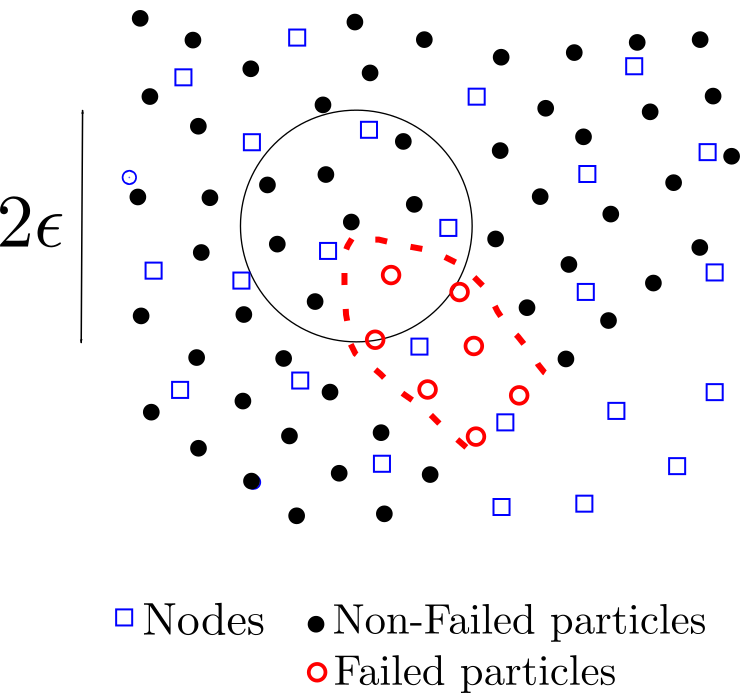
\includegraphics[width=\textwidth]{./Figures/Discretization_MPM}
  }
  \caption{MPM discretization.}
  \label{fig:MPM-discretization}
\end{figure}

Each material point is assigned with initial values of position,
velocity, mass, volume and stress denoted by $\vec{x}_p$,
$\vec{v}_p$, $m_p$,  $V_p$ and $\tens{\sigma}_p$, but also the
virtual field $\vect{v}^{\psi}_{p}$. So employing the definition of the
material integral, where we recover the Riemann integral definition as
an addition  of a finite set of points. Therefore individual terms in
\eqref{eq:BalanceMomentum_wf} are solved as follows. 
\begin{itemize}
\item Acceleration forces :
\begin{equation}
    \label{eq:particle_acceleration_forces}
    \Integral{3}{\rho\ \vec{a} \cdot \vect{v}^{\psi}} =
    \dot{\vec{v}}_{p} \cdot \vect{v}^{\psi}_{p}\ m_p.
  \end{equation}\\
\item Internal forces :
  \begin{equation}
    \label{eq:particle_internal_forces}
    \Integral{3}{\tens{\sigma}\ \colon \tens{\varepsilon}^{\psi}} =
   \tens{\sigma}_{p}\ \colon \tens{\varepsilon}^{\psi}_p \ V_p.
  \end{equation}\\
\item Body forces :
\begin{equation}
  \label{eq:particle_body_forces}
  \Integral{3}{\rho\ \vec{b} \cdot \vect{v}^{\psi} } = 
  \vec{b}_{p} \cdot \vect{v}^{\psi}_p\ m_p.
\end{equation}\\
\item Loads :
\begin{equation}
  \begin{aligned}
    \label{eq:particle_load_forces}
    \Integral{2}{\vec{t}\ \vect{v}^{\psi}} = \Integral{2}{\rho\
      \vec{t}^s \cdot \vect{v}^{\psi}} = \vec{t}^s_{p} \cdot \vect{v}^{\psi}_{p}\ h^{-1}\ m_p ,
  \end{aligned} 
\end{equation}
\end{itemize}
where $h$ is the thickness of the continuum in a 2D case. Here is
where the second discretization procedure appears. A background mesh
composed by a finite set of grid points with coordinates $\vec{x}_I\
, I = 1,2\ldots ,N_n$, is generated. Where $N_n$ is the number of grid
nodes. This mesh is employed as a support to compute gradients and divergences. 

Introducing \eqref{eq:particle_acceleration_forces},
\eqref{eq:particle_internal_forces}, \eqref{eq:particle_body_forces}, 
and \eqref{eq:particle_load_forces} in \eqref{eq:BalanceMomentum_wf},
and approximating the real and virtual velocity  field of the particle
$p$ as
\begin{equation}
  \label{eq:Approx-velocity-mesh}
  \vec{v}_{p} = N_I(\vec{x}_p) \vect{v}_I
  \quad \text{and} \quad \vec{v}^{\psi}_{p} = N_I(\vec{x}_p) \vect{v}_I^{\psi},
\end{equation}
\begin{equation}
  \label{eq:Approx-gradvelocity-mesh}
  \Grad{\vect{v}}_p = \vect{v}_I N_I(\vec{x}_p)
  \quad \text{and} \quad \vec{v}^{\psi}_{p} = \sum^{Nn}_I N_I(\vec{x}_p) \vect{v}_I^{\psi},
\end{equation}
we reach to the particle balance of forces of the continuum,
\begin{equation}
  \label{eq:particle_balance_forces3}
  \dot{\vec{p}}_{I}= \tens{m}_{IJ}\dot{\vec{v}}_{J} = \vec{f}_{I}^{int} + \vec{f}_{I}^{ext},
\end{equation}
where $\dot{\vec{p}}_{I}$ is the rate of momentum at grid node $I$, the nodal mass matrix $\tens{m}_{IJ}$ is,
\begin{equation}
  \label{eq:particle_nod_mass}
  \tens{m}_{IJ} =
  \sum^{Np}_{p} N_{Ip} m_p N_{Jp}.
\end{equation}
To improve the computational efficiency and stability, the nodal mass matrix
\eqref{eq:particle_nod_mass} can be substituted by the lumped mass
matrix $\tens{m}_{IJ}^{lumped}$.
Later, internal and external forces are computed as follows,
\begin{equation}
  \label{eq:nodal_internal_forces}
  \vec{f}_{I}^{int} = - \sum^{N_p}_{p} \tens{\sigma}_{p} \cdot \Grad{N_{Ip}} \frac{m_p}{\rho_p}
\end{equation}
\begin{equation}
  \label{eq:nodal_external_forces}
  \vec{f}_{I}^{ext} = \sum^{N_p}_{p} N_{Ip} \vec{b}_{p} m_p  + \sum^{N_p}_{p}
  N_{Ip} \vec{t}^s_{p} m_p h^{-1} 
\end{equation}
where $\tens{\sigma}_{p} = \tens{\sigma}_{p}(\tens{\varepsilon}_{p})$
is the particle $p$ stress field, which can be integrated employing
the suitable constitutive model. The strain tensor is updated employing the rate of stress tensor $\dot{ \tens{\varepsilon}}_{p}$ used to update the
strain tensor is as follows \eqref{eq:IncrStrainPoint}.
\begin{equation}
  \label{eq:IncrStrainPoint}
  \dot{\tens{\varepsilon}_{p}} = \frac{\Delta
    \tens{\varepsilon}_{p}}{\Delta t} =
  \frac{1}{2} \sum^{Nn}_I \left[\Grad{N_{Ip}}\ \otimes \vec{v}_{I} + \vec{v}_{I} \otimes
    \Grad{N_{Ip}}\ \right].
\end{equation}
Next, imposing $\frac{D \rho}{D t} = 0$, we ensures the mass
conservation and update the density field.
\begin{equation}
  \label{eq:MassConservation}
\dot{\rho} = - \rho\ \mathit{tra} \left( \dot{\tens{\varepsilon}} \right)
\end{equation}

Finally, to solve the equation \eqref{eq:particle_balance_forces3}, a second order
temporal integration scheme is required. Therefore, time is
discretized in to a finite set of time steps $k = 1\ldots ,Nt$, where $k$ is the current time step and $N_t$
is the total number of time steps. Once the nodal equilibrium equation it is solved, the values in the nodes are
interpolated back in to the particles and each particle it is advected
to the new position,
\begin{equation}
  \label{eq:Updated_Lagrangian}
  \dot{\vec{v}}_p = \sum^{N_n}_{I}N_{Ip}\ \vec{a}_{I},\quad and\quad
  \dot{\vec{x}}_{p} = \sum^{N_n}_{I}N_{Ip}\ \vec{v}_{I}  
\end{equation}
In the MPM literature, this equations
(\ref{eq:particle_balance_forces3}) and (\ref{eq:Updated_Lagrangian}),
are solved with an explicit forward Euler algorithm. The time integration scheme of the MPM has been described in detail by many researchers
\cite{Sulsky1994}, \cite{Bardenhagen2002}, \cite{thesis_Andersen_2009} and summarized
in Figure \ref{fig:MPM_algorithm}.

\begin{figure}\sidecaption
  \centering
  \resizebox{0.55\hsize}{!}{
    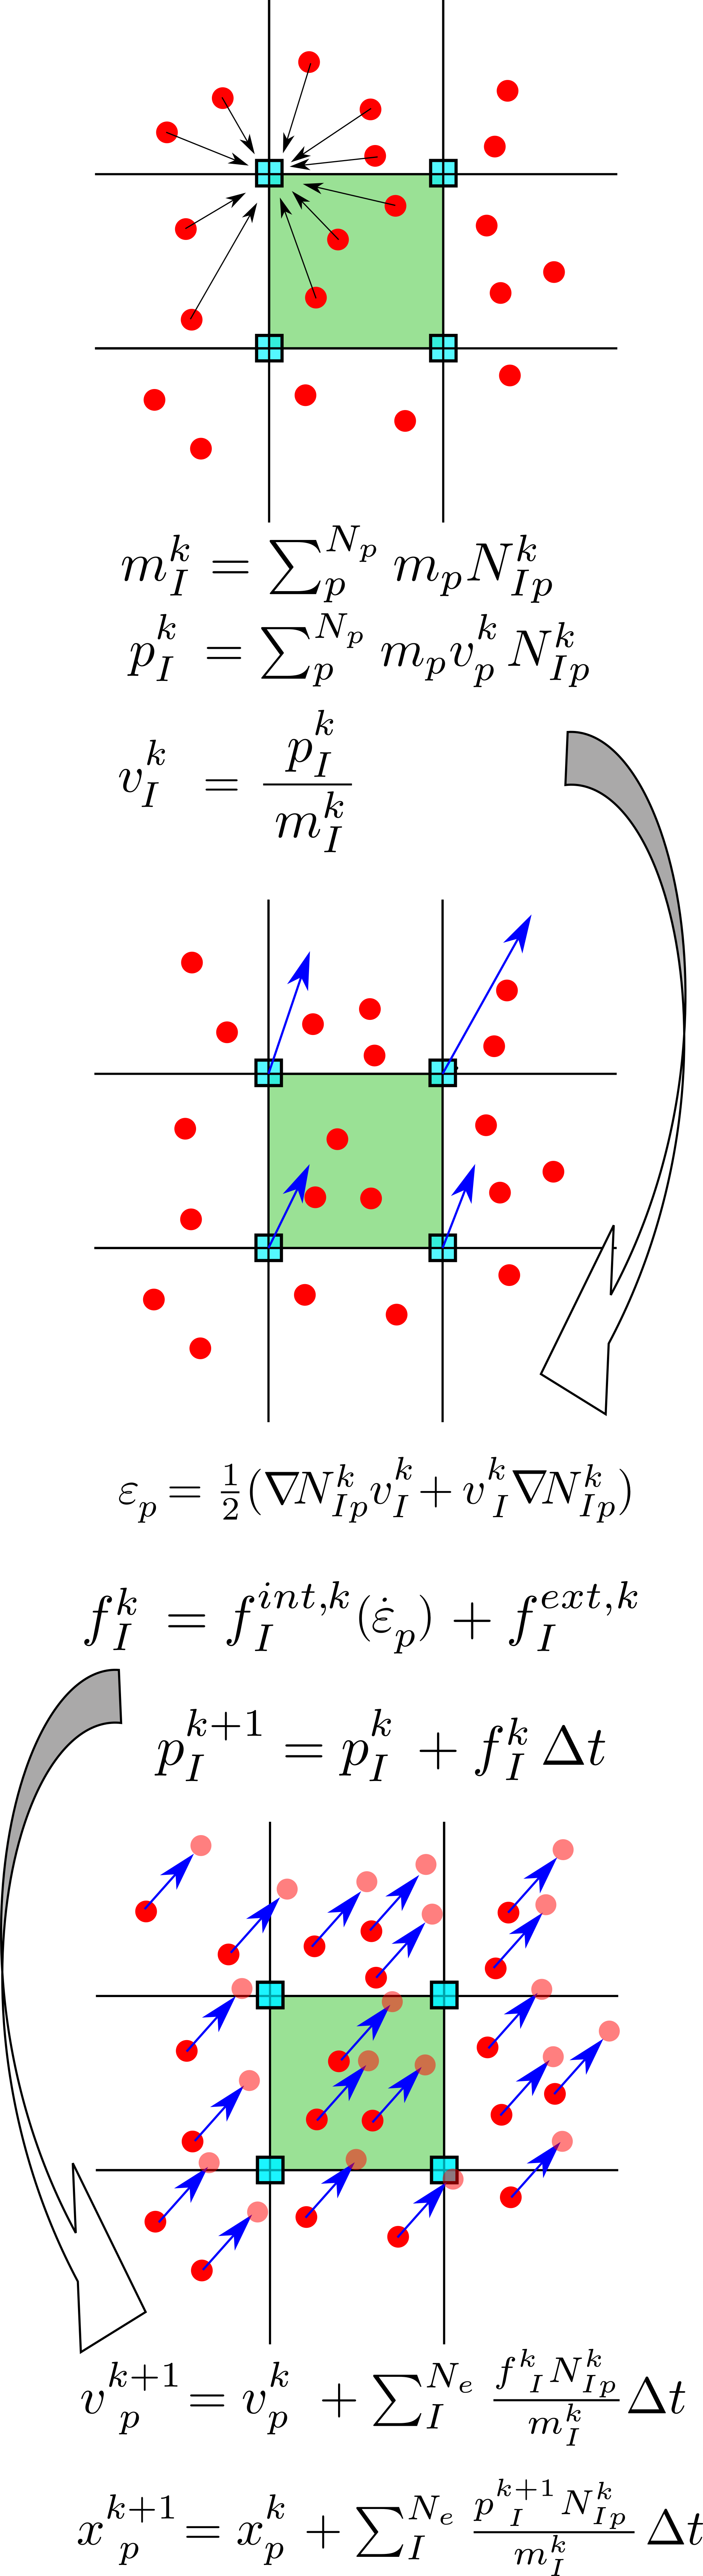
\includegraphics[width=\textwidth]{./Figures/MPM_scheme}
  }
  \caption{MPM standard algorithm.}
  \label{fig:MPM_algorithm}
\end{figure}

Other authors have proposed many others time integration alternatives
like \cite{Guilkey2003}, \cite{Tran2019e}, \cite{Charlton2017}. In the
first publication on the MPM \cite{Sulsky1994}, the nodal acceleration
was employed to update the particles as
\begin{equation}
  \label{eq:Sulsky-1994-UL-v}
  \vect{v}_p^{k+1} = \vect{v}_p^{k} + \Delta t\
  \sum^{N_n}_{I}N_{Ip}^{k}\ \vec{a}_{I}^{k}
\end{equation}
\begin{equation}
  \label{eq:Sulsky-1994-UL-x}
  \vect{x}_p^{k+1} = \vect{x}_p^{k} + \Delta t\ \sum^{N_n}_{I}N_{Ip}^{k}\ \vec{v}_{I}^{k}.
\end{equation}
However, as Andersen (2009)\cite{thesis_Andersen_2009} point out, this algorithm has been shown to be numerically unstable due to that
$\vect{f}_I^{int,k}$ can be finite for an infinitesimal nodal mass
$\tens{m}$. This can lead to numerical issues when nodal acceleration
is obtained for evaluating \eqref{eq:Sulsky-1994-UL-x},\eqref{eq:Sulsky-1994-UL-v}. Hence, a
corrected version of this algorithm in shown in Zhang {\it et al.}
(2016)\cite{Zhang_book_2016}
\begin{equation}
  \label{eq:Zhang-2016-UL-x}
  \vect{x}_p^{k+1} = \vect{x}_p^{k} + \Delta t\ \sum^{N_n}_{I} \frac{N_{Ip}^{k}\ \vec{p}_{I}^{k}}{\tens{m}_I}.  
\end{equation}
\begin{equation}
  \label{eq:Zhang-2016-UL-v}
  \vect{v}_p^{k+1} = \vect{v}_p^{k} + \Delta t\
  \sum^{N_n}_{I}\frac{N_{Ip}^{k}\ \vec{f}_{I}^{k}}{\tens{m}_I},
\end{equation}
Later Tran \& Solowski (2019)\cite{Tran2019e} presented a
generalized-$\alpha$ scheme for the MPM inspired in the explicit time
integration algorithm proposed by Chung \& Hulbert
(1993)\cite{Geranlized_alpha_1993}, but with the particularity that
the acceleration is evaluated both in the beginning and the end of the
time step.
\begin{equation}
  \label{eq:Tran-2019-GA-v}
  \vect{v}_p^{k+1} = \vect{v}_p^{k} + \Delta t\
  \sum^{N_n}_{I} N_{Ip}^{k}\ \left[(1 - \gamma)\ \vect{a}_I^{k} +
    \gamma\ \vect{a}_I^{k+1} \right],\\
\end{equation}
\begin{equation}
\label{eq:Tran-2019-GA-x}
  \vect{x}_p^{k+1} = \vect{x}_p^{k} + 
  \sum^{N_n}_{I}N_{Ip}^{k} \left[ \Delta t\ \vec{v}_{I}^{k}+ \Delta t^2\left( (\frac{1}{2} - \beta)\
    \vec{a}_{I}^{k} + \beta\ \vec{a}_{I}^{k+1} \right) \right]
\end{equation}
\begin{equation}
  \label{eq:Tran-2019-GA-a}
  \vect{a}_p^{k+1} = \sum^{N_n}_{I}N_{Ip}^{k}\ \vec{a}_{I}^{k+1}.
\end{equation}

This scheme has prof to damps out the higher frequency noises
\cite{Tran2019e}. But it can present the same numerical instabilities
as in \eqref{eq:Sulsky-1994-UL-x},\eqref{eq:Sulsky-1994-UL-v} when
nodal masses become infinitesimal.

\section{Explicit predictor-corrector scheme for MPM.}
\label{sec:epc-algor-mpm}

In this section, an explicit predictor-corrector time integration
scheme is presented. It is based in the Newmark a-form 
$\gamma = 0.5$ and $\beta = 0$ which is the central difference
explicit. This method is devoted to solve a system of equations of type
\begin{equation*}
  \Matrix{M}_{IJ}\ddot{\Vector{d}}_{J} + \Matrix{C}_{IJ}\dot{\Vector{d}}_{J} +
  \Matrix{K}_{IJ}\Vector{d}_{J} = \Vector{F}_{I}.
\end{equation*}

As the MPM has a nodal stage, it is possible to apply this methods
successfully in the MPM framework as was proved by
\cite{Tran2019e}. Taking the predictor definition from the classic
literature \cite{Hughes2000} and calculating nodal velocity, and
updating particles position employing nodal values of velocity and
acceleration. Therefore we get the following expression for the
\textbf{predictor} stage for both velocity and displacement.
\begin{equation}
  \label{eq:5}
  \vec{x}_p^{k+1} = \vec{x}_p^n + \Delta t\
  \underbrace{\sum^{N_n}_{I}N_{Ip}^k\ \vec{v}_{I}^{k}}_{\vec{v}_p^{k}} + \frac{1}{2}\Delta
  t^2\ \underbrace{\sum^{N_n}_{I}\frac{N_{Ip}^k\ \vec{f}_{I}^{k}}{\tens{m}_I^k}}_{\vec{a}_p^{k}}
\end{equation}
\begin{equation}
  \label{eq:Predictor-velocity}
  \vec{v}_I^{k+1} = \vec{v}_I^n + (1 - \gamma)\ \Delta t\ \vec{a}_I^k
  \quad , \quad \vec{a}_I^k = \frac{\vec{f}_{I}^{k}}{\tens{m}_I^k}
\end{equation}

Consequently, the \textbf{corrector} stage for the nodal velocity is in the
following way
\begin{equation}
  \vec{v}_{I}^{k+1} = \vec{v}_{I}^{k+1} + \gamma\ \Delta t\
  \vec{a}_I^{k+1} \quad , \quad  \vec{a}_I^{k+1} = \frac{\vec{f}_{I}^{k+1}}{\tens{m}_I^{k+1}} 
\end{equation}

Notice that the predictor of the particle displacement is
computed using information only from the predictor of the
previous step. However, velocities are computed using half information
of the past corrector and half of the past predictor. Therefore here we share
similarities with the \textbf{leapfrog integration} which updates the
position at full time step, but updates the velocity at half time
steps. Notice also that with this approach the calculation of nodal
momentum vales in not required, and particles velocities is just a
post-process. So during the lagrangian step only the particles
position is truly computed. This minimizes the information
transference between the particles and nodes, and in consequence
minimizes the associated error to this process. 

Due to its simplicity allows be implemented with minor modifications
over a standard forward Euler. It is summarized in shape of
pseudo-algorithm \ref{alg:PCE-algorithm}.

\begin{algorithm}
  \label{alg:PCE-algorithm}
  \floatname{algorithm}{Algorithm}
  \renewcommand{\thealgorithm}{}
  \caption{Explicit Predictor-Corrector scheme}
  \begin{algorithmic}[1]
    %%%%%%%%%%%%%%%%%%%%%%%%%%%%%%%%%%%%%%%%%%%%%%%%%%%%%%%%%%%%%%%%%%%%%%%%%%%%%%%%%%%%%% º
    \STATE \textbf{Explicit Newmark Predictor} ($\gamma = 0.5$):\\
    Only in those active nodes:
    \begin{equation*}
      \vec{v}_I^{k+1} = \vec{v}_I^n + (1 - \gamma)\ \Delta t\ \vec{a}_I^k
      \quad , \quad \vec{a}_I^k = \frac{\vec{f}_{I}^{k}}{\tens{m}_I^k}
    \end{equation*}
    %%%%%%%%%%%%%%%%%%%%%%%%%%%%%%%%%%%%%%%%%%%%%%%%%%%%%%%%%%%%%%%%%%%%%%%%%%%%%%%%%%%%%% 
    \STATE \textbf{Impose essential boundary conditions}:\\
    At the fixed boundary, set $\vec{v}_{I}^{k+1} = 0$. 
    %%%%%%%%%%%%%%%%%%%%%%%%%%%%%%%%%%%%%%%%%%%%%%%%%%%%%%%%%%%%%%%%%%%%%%%%%%%%%%%%%%%%%% 
    % \STATE \textbf{Discard the previous nodal values}.
    %%%%%%%%%%%%%%%%%%%%%%%%%%%%%%%%%%%%%%%%%%%%%%%%%%%%%%%%%%%%%%%%%%%%%%%%%%%%%%%%%%%%%% 
    \STATE \textbf{Update mass matrix}:
    \begin{equation*}
      \tens{m}_{I} = \sum_{p}^{N_p}N_{Ip}^{k+1}\ m_p,
    \end{equation*}
    %%%%%%%%%%%%%%%%%%%%%%%%%%%%%%%%%%%%%%%%%%%%%%%%%%%%%%%%%%%%%%%%%%%%%%%%%%%%%%%%%%%%%% 
    \STATE \textbf{Deformation tensor increment calculation}.
    \begin{align*}
      &\dot{\tens{\varepsilon}_{p}}^{k+1} = \frac{1}{2}\ \sum_{I}^{N_n}
        \Grad{N_{Ip}^{k+1}}\vec{v}_{I}^{k+1} +
        (\Grad{N_{Ip}^{k+1}}\vec{v}_{I}^{k+1})^T \\
      &\Delta \tens{\varepsilon}_{p}^{k+1} = \Delta t\ \dot{\tens{\varepsilon}_{p}}^{k+1}
    \end{align*}
    %%%%%%%%%%%%%%%%%%%%%%%%%%%%%%%%%%%%%%%%%%%%%%%%%%%%%%%%%%%%%%%%%%%%%%%%%%%%%%%%%%%%%% 
    \STATE \textbf{Update the density field}:
    \begin{equation*}
      \rho_p^{k+1} = \frac{\rho_p^k}{1 + \mathit{tra}\left[\Delta\tens{\varepsilon}_{p}^{k+1}\right]}.
    \end{equation*}
    %%%%%%%%%%%%%%%%%%%%%%%%%%%%%%%%%%%%%%%%%%%%%%%%%%%%%%%%%%%%%%%%%%%%%%%%%%%%%%%%%%%%%% 
    \STATE \textbf{Balance of forces calculation}:\\
    Calculate the total grid nodal force $\vec{f}_{I}^{k+1} =
    \vec{f}_{I}^{int,k+1} + \vec{f}_{I}^{ext,k+1}$ evaluating
    \eqref{eq:nodal_internal_forces} and \eqref{eq:nodal_external_forces} in the time step $k+1$. In the
    grid node $I$ is fixed in one of the spatial dimensions, set it to
    zero to make the grid nodal acceleration zero in that direction.\\
    %%%%%%%%%%%%%%%%%%%%%%%%%%%%%%%%%%%%%%%%%%%%%%%%%%%%%%%%%%%%%%%%%%%%%%%%%%%%%%%%%%%%%% 
    \STATE \textbf{Explicit Newmark Corrector} ($\gamma = 0.5$):
    \begin{equation*}
      \vec{v}_{I}^{k+1} = \vec{v}_{I}^{k+1} + \gamma\ \Delta t\
      \vec{a}_I^{k+1} \quad , \quad  \vec{a}_I^{k+1} = \frac{\vec{f}_{I}^{k+1}}{\tens{m}_I^{k+1}}  
    \end{equation*}
    %%%%%%%%%%%%%%%%%%%%%%%%%%%%%%%%%%%%%%%%%%%%%%%%%%%%%%%%%%%%%%%%%%%%%%%%%%%%%%%%%%%%%%
    \STATE \textbf{Update particles position and velocity}:
    \begin{align*}
      &\vec{x}_p^{k+1} = \vec{x}_p^n + \Delta t\
        \sum^{N_n}_{I} N_{Ip}^k\ \vec{v}_{I}^{k} +
        \frac{1}{2}\Delta t^2\ \sum^{N_n}_{I}\frac{N_{Ip}^k\
        \vec{f}_{I}^{k}}{\tens{m}_I^k}\\
      &\vec{v}_p^{k+1} = \vec{v}_p^n + \Delta t\
        \sum^{N_n}_{I}\frac{N_{Ip}^k\
        \vec{f}_{I}^{k}}{\tens{m}_I^k}
    \end{align*}
  \end{algorithmic}
\end{algorithm} 

\section{Local max-ent approximants}
\label{sec:local-max-ent}

% The previous lines describe the main algorithm without defining an
% interpolation technique, so we are free to apply a wide range of the
% existing. 

The popularity of the MPM has increase notoriously during
the recent years due to its ability to deal with large strain problems
without mesh distorsion issues inherent to mesh based methods like
FE, see Zdzislaw \cite{Wieckowski2004}. However, in the simulations made with the original MPM, there are
numerical noises when particles crossing the cell boundaries. Recently
the local maximum-entropy (or local \textit{max-ent}) shape function
first introduced by Arroyo \& Ortiz (2006)\cite{Arroyo2006} has been
tested under the MPM framework by Wobbes {\it et al.} (2020)\cite{Wobbes2020} where they prof that
simulations performed with the maxent basis functions show
considerably more accurate stress approximations for MPM. Although, in
\cite{Wobbes2020} authors does not deep in how $\beta$ affects to the
accuracy and stability of the solution.

The basic idea of the shape functions based on such
an estimate is to interpret the shape function $N_I(\vec{x})$ as the
probability of $\vec{x}$ to obtain the value $\vec{x}_I$,  $I=1,
\dots, n$. Here $n$ is the number of nodes in the domain.

Taking the definition of entropy as a measure of how uncertainty a
random variable is averaged on all its possible outcomes. 

Therefore following the principle of \textit{maximum-entropy}
stated by Jaynes \cite{Jaynes1957}, the least biased shape functions
are those that maximizes the entropy of the scheme

estimate is defined as the type of statistical
inference, which is the least biased possible on the given information.

Taking Shannon's entropy as the starting point:
\begin{equation}
  \label{eq:Shannon-entropy}
  H(p_1(\vec{x}),\ldots,p_n(\vec{x})) = -\sum^{N_n}_{I=1}{p_I(\vec{x})\log p_I }
\end{equation}
where $p_I(\vec{x})$ is the probability, equivalent to the mentioned
shape function $N_I(\vec{x})$,  satisfying both the zeroth and
first-order consistency.

The least-biased approximation scheme is given by
\begin{align*}
  \text{(LME)} \hspace{0.15cm} \text{Maximize} \hspace{0.15cm} &H(p) = -\sum_{I}^{N_n}{p_I(\vec{x})\log p_I } \nonumber \\
  \text{subject to} \hspace{0.15cm} &p_I \ge 0, \hspace{0.15cm} \text{I=1, ..., n} \nonumber \\
  &\sum_{I=1}^{N_n}{p_I} = 1 \nonumber \\
  &\sum_{I=1}^{N_n}{p_I \vec{x}_I} = \vec{x} \nonumber 
\end{align*}

The local max-ent approximation schemes (LME) as a Pareto set,
defined by \cite{Arroyo2006} is as follows 
\begin{align*}
  \text{(LME)}_{\beta} \hspace{0.15cm} \text{For fixed} \hspace{0.15cm}
  \vec{x} \hspace{0.15cm} \text{minimise}  \nonumber \hspace{0.15cm} &f_{\beta}(\vec{x}, p) = \beta H(\vec{x},p) - H(p) \\
  \text{subject to} \hspace{0.15cm} &p_I \ge 0, \hspace{0.2cm} \text{I=1, ..., n}  \\
                                                                   &\sum_{I=1}^{N_n}{p_I} = 1 \\
                                                                   &\sum_{I=1}^{N_n}{p_I \, \vec{x}_I} = \vec{x}
\end{align*}
for $\beta \in (0,\infty)$ is Pareto optimal. The unique solution of
the local max-ent problem (LME)$_\beta$ is: 
\begin{equation}
  \label{eq:LME-p}
p(\vec{x})=\frac{\exp\left[ -\beta \; |\vec{x}-\vec{x}_I|^2 +  \vec{\lambda}  \;  (\vec{x}-\vec{x}_I)         \right] } {Z(\vec{x},\vec{\lambda}^*(\vec{x}))}
\end{equation}
where
\begin{equation}
  \label{eq:LME-Z}
Z(\vec{x}, {\vec{\lambda}}) = \sum_{I=1}^{N_n}{ \exp \left[ -\beta \, | \vec{x}-\vec{x}_I|^2 + \vec{\lambda}  \,  (\vec{x}-\vec{x}_I)  \right]}
\end{equation}
being $\vec{\lambda}^*(\vec{x})$ the unique minimiser  for $\log Z(\vec{x}, \vec{\lambda})$

In order to obtain the first derivatives of the shape function, it is  also necessary to compute~$\nabla p^*_I$ 
\begin{equation}
  \label{eq:LME-grad-p}
\nabla p^*_I=p^*_I  \, \left(\nabla f^*_I-\sum_J^{N_n} p^*_J \, \nabla f^*_J\right)
\end{equation}
where
\begin{equation}
  \label{eq:LME-f}
f^*_I(\vec{x},  \vec{\lambda},\beta)=-\beta \, |\vec{x}-\vec{x}_I|^2 + \vec{\lambda}   \,  (\vec{x}-\vec{x}_I)
\end{equation}
Employing the chain rule, rearranging and considering $\beta$ as a constant, Arroyo and Ortiz~\cite{Arroyo2006} obtained the following expression:
\begin{eqnarray}
\nabla p^*_I &=& -p^*_I \,  (\tens{J}^*)^{-1} \,  (\vec{x} - \vec{x}_I) \label{eq26} 
\end{eqnarray}
%&&\mbox{
where \tens{J} is the Hessian matrix, defined by:
%} \nonumber \\&& \nonumber \\
\begin{eqnarray}
\tens{J}(\vec{x},  \vec{\lambda},\beta) &=& \frac{\partial \vec{r}}{\partial  \vec{\lambda}} \label{eq27} \\ 
%&& \nonumber \\
\vec{r}(\vec{x},\vec{\lambda},\beta) &\equiv& \partial_{\vec{\lambda}}{\log{ Z( \vec{x},\vec{\lambda}})} 
%\nonumber \\ &=&
  =\sum_I^{N_n} p_I(\vec{x},\vec{\lambda},\beta) \, (\vec{x} - \vec{x}_I) \label{eq28} 
\end{eqnarray}
Note that, the objective of the above procedure is to find the
$\vec{\lambda}$ which minimises  $\log Z(\vec{x}, \vec{\lambda})$. The
traditional way to obtain such a minimiser  is using Eq.~(\ref{eq27})
to calculate small increments of $\partial\vec{\lambda}$ in a
Newton-Raphson approach.

Similar to alternative non-polynomial meshfree basis functions, the
LME approximation scheme requires more than $d+1$ nodes to determine
the values of the shape functions as well as their derivatives at any
point in the convex hull of the nodal set, where $d$ is the dimension
of the problem. Due to the FE-compatibility, the LME shape function is
degenerated to linear finite element shape function if $d+1$
neighbouring nodes are chosen as the support. The support size of LME
shape functions may be controlled by adjusting a dimensionless
parameter, $\gamma=\beta h^2$ (e.g. two dimensional example shown in
figure. \ref{fig:LME_MPM})\cite{Arroyo2006}.


\begin{figure}
  \centering
  %%%%%%%%%%%%%%%%%%%%%%%%%%%%%%%%%%%%%%%%%%%%%% 
  \subfloat[Piecewise linear (Q4).]{
    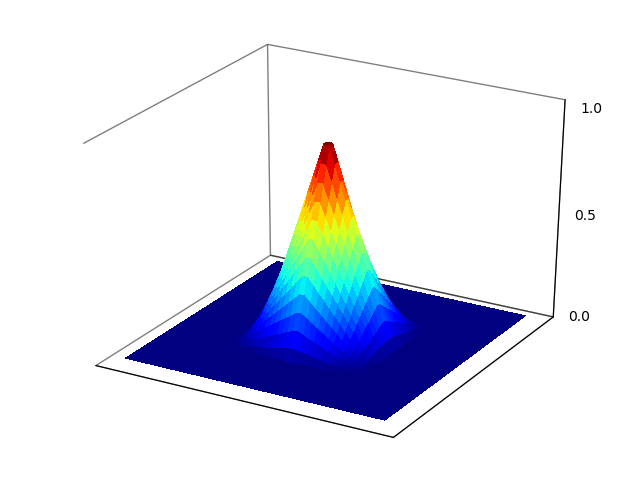
\includegraphics[width=0.3\columnwidth]{Figures/MPM_Shape_Fun}
    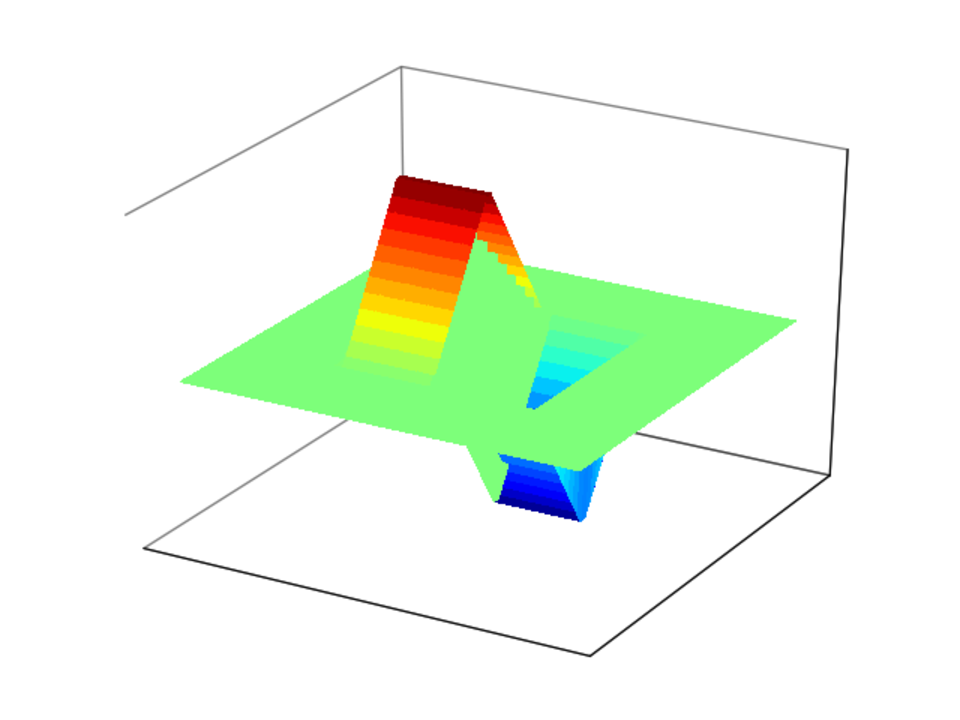
\includegraphics[width=0.3\columnwidth]{Figures/MPM_Shape_Fun_dx}
    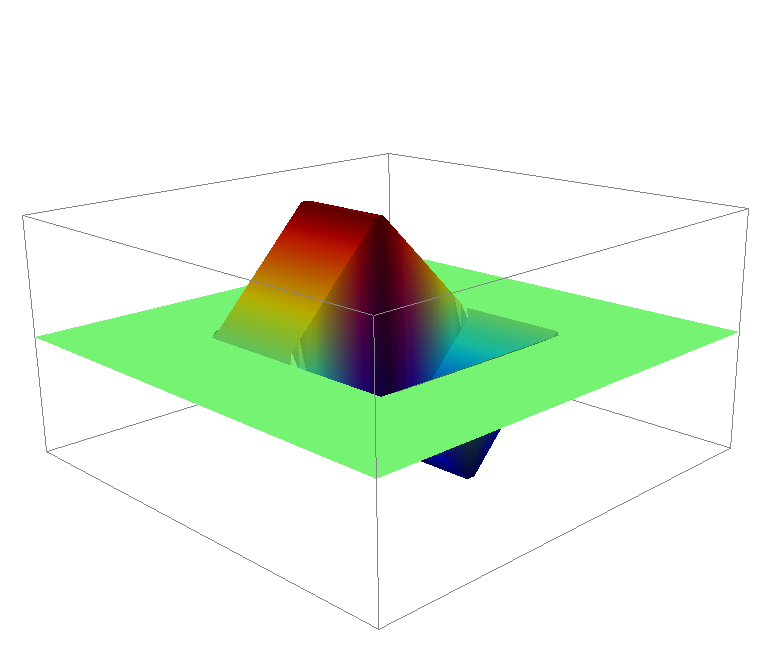
\includegraphics[width=0.3\columnwidth]{Figures/MPM_Shape_Fun_dy}
    \label{fig:MPM_Shape_Fun}
  }
  %%%%%%%%%%%%%%%%%%%%%%%%%%%%%%%%%%%%%%%%%%%%%% 
  \qquad
  %%%%%%%%%%%%%%%%%%%%%%%%%%%%%%%%%%%%%%%%%%%%%% 
  \subfloat[Local \textit{max-ent} $\gamma=17$.]{
    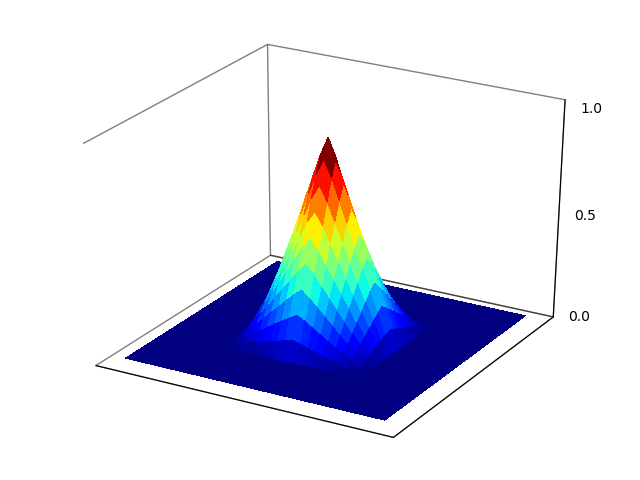
\includegraphics[width=0.3\columnwidth]{Figures/LME_17_3_Shape_Fun}
    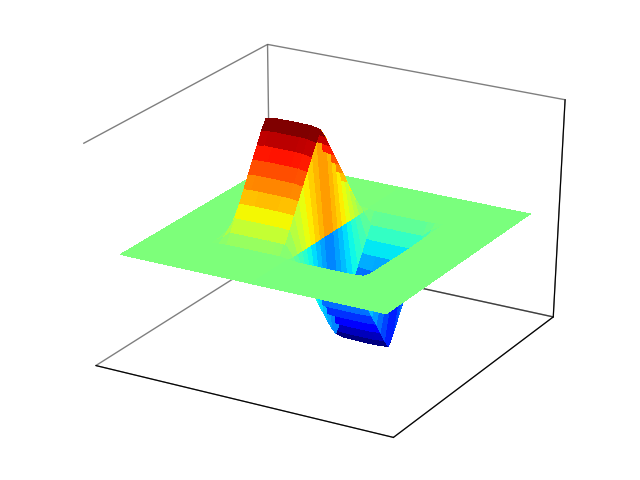
\includegraphics[width=0.3\columnwidth]{Figures/LME_17_3_Shape_Fun_dx}
    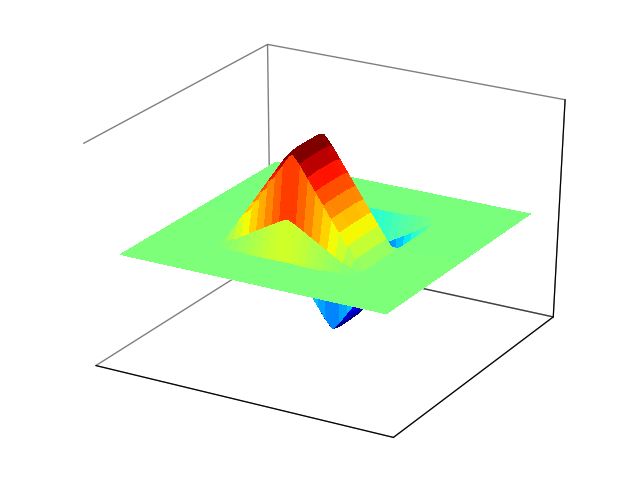
\includegraphics[width=0.3\columnwidth]{Figures/LME_17_3_Shape_Fun_dy}
    \label{fig:LME_17.3_Shape_Fun}
  }
  %%%%%%%%%%%%%%%%%%%%%%%%%%%%%%%%%%%%%%%%%%%%%% 
  \qquad
  %%%%%%%%%%%%%%%%%%%%%%%%%%%%%%%%%%%%%%%%%%%%%% 
  \subfloat[Uniform generalized interpolated material point.]{
    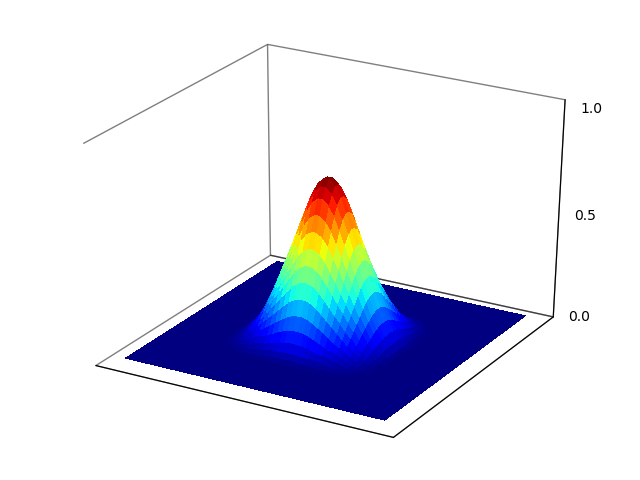
\includegraphics[width=0.3\columnwidth]{Figures/GIMP_Shape_Fun}
    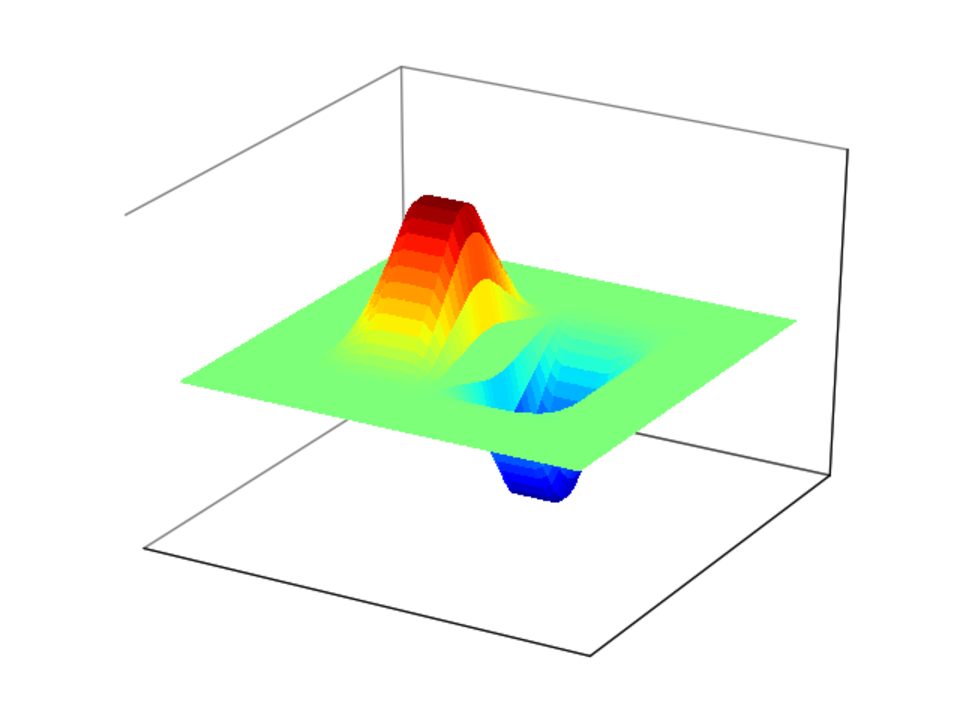
\includegraphics[width=0.3\columnwidth]{Figures/GIMP_Shape_Fun_dx}
    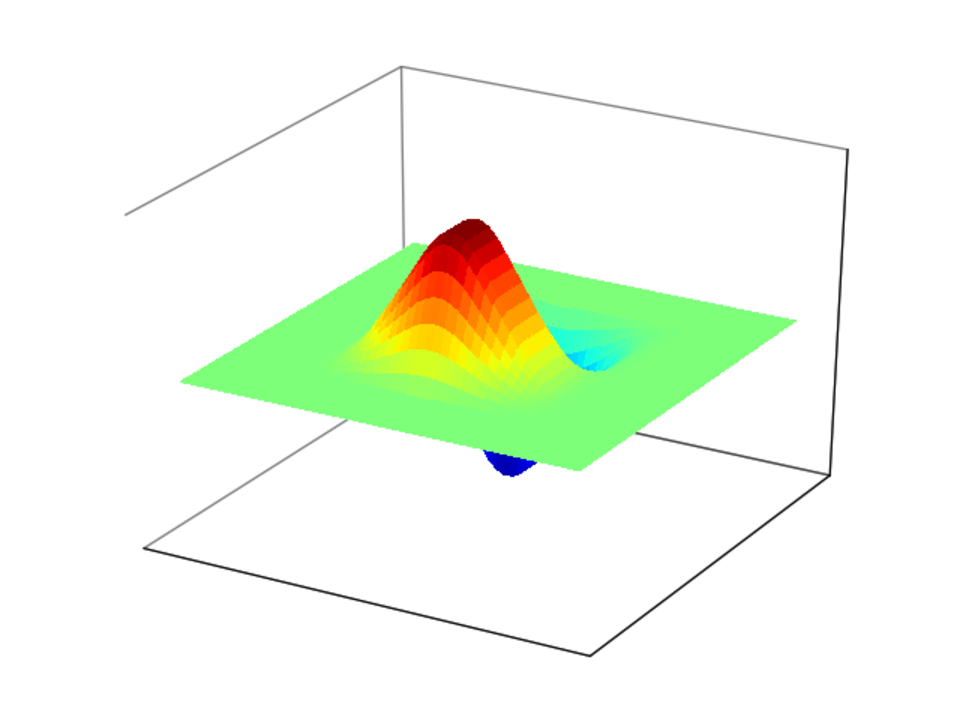
\includegraphics[width=0.3\columnwidth]{Figures/GIMP_Shape_Fun_dy}
    \label{fig:GIMP_Shape_Fun}
  }
  %%%%%%%%%%%%%%%%%%%%%%%%%%%%%%%%%%%%%%%%%%%%%% 
  \qquad
  %%%%%%%%%%%%%%%%%%%%%%%%%%%%%%%%%%%%%%%%%%%%%%
  \subfloat[Local \textit{max-ent} $\gamma=10$.]{
    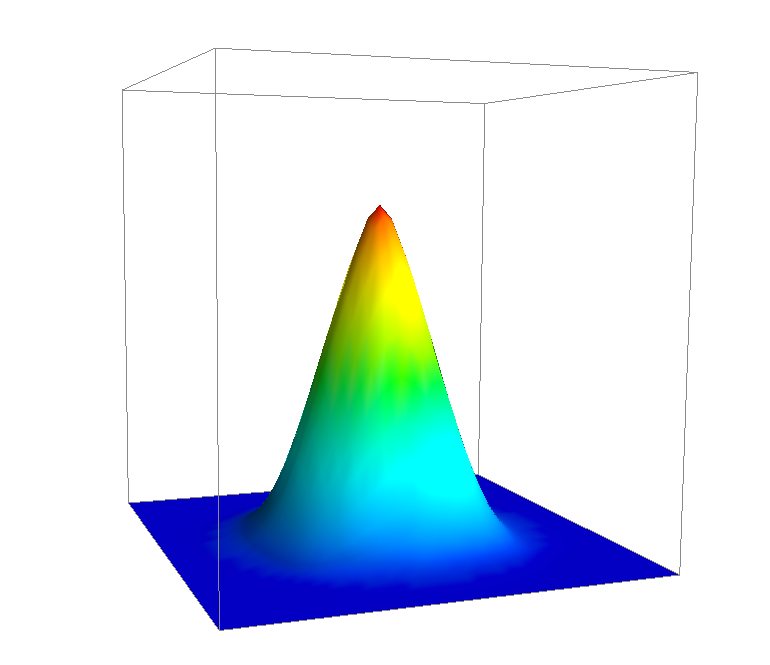
\includegraphics[width=0.3\columnwidth]{Figures/LME_10_0_Shape_Fun}
    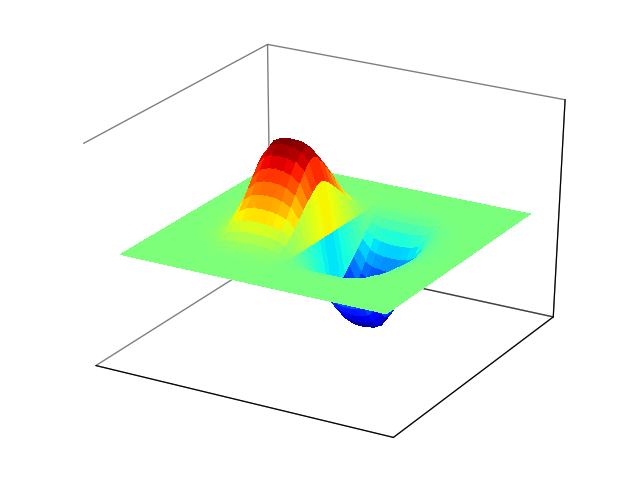
\includegraphics[width=0.3\columnwidth]{Figures/LME_10_0_Shape_Fun_dx}
    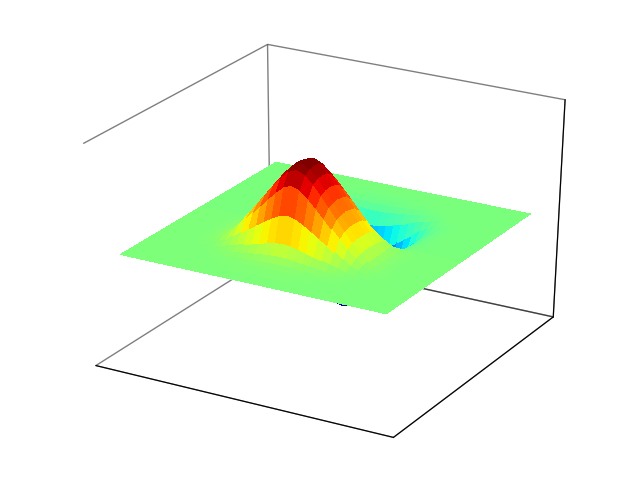
\includegraphics[width=0.3\columnwidth]{Figures/LME_10_0_Shape_Fun_dy}
    \label{fig:LME_10.0_Shape_Fun}
  }
  %%%%%%%%%%%%%%%%%%%%%%%%%%%%%%%%%%%%%%%%%%%%%% 
  \qquad
  %%%%%%%%%%%%%%%%%%%%%%%%%%%%%%%%%%%%%%%%%%%%%%  
  \subfloat[Local \textit{max-ent} $\gamma=7$.]{
    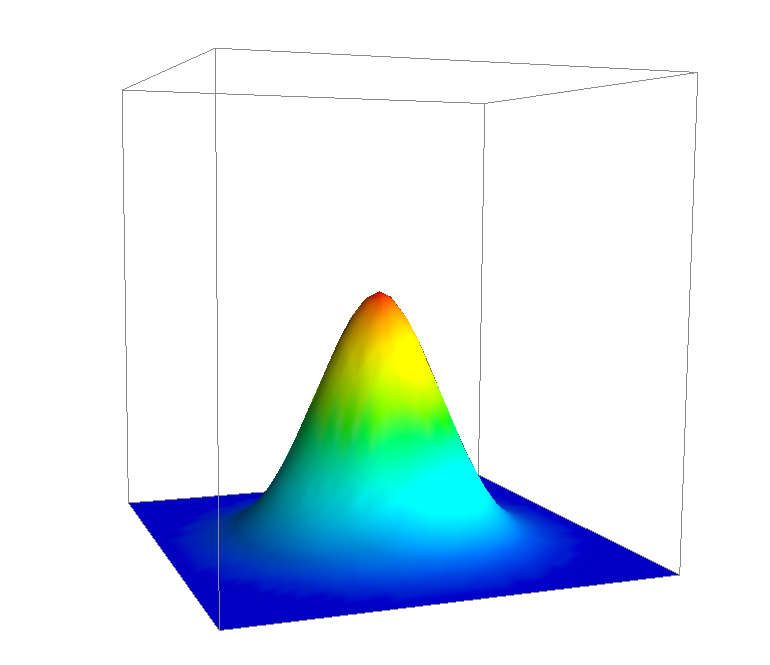
\includegraphics[width=0.3\columnwidth]{Figures/LME_7_0_Shape_Fun}
    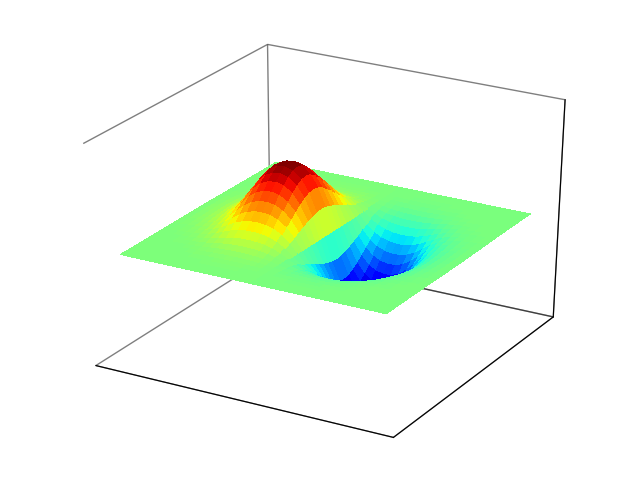
\includegraphics[width=0.3\columnwidth]{Figures/LME_7_0_Shape_Fun_dx}
    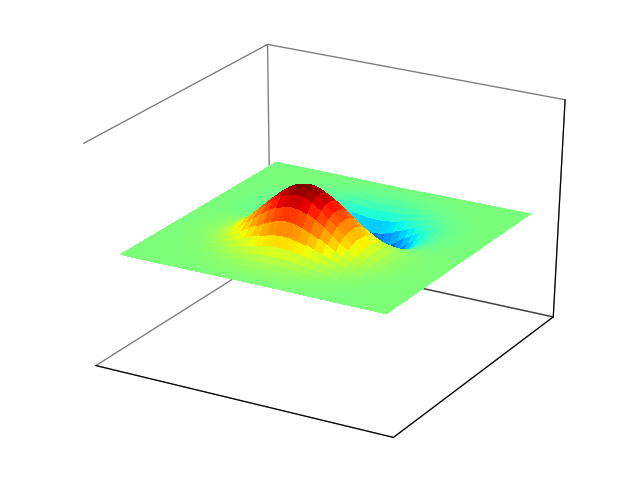
\includegraphics[width=0.3\columnwidth]{Figures/LME_7_0_Shape_Fun_dy}
    \label{fig:LME_7.0_Shape_Fun}
  }
  %%%%%%%%%%%%%%%%%%%%%%%%%%%%%%%%%%%%%%%%%%%%%% 
  \qquad
  %%%%%%%%%%%%%%%%%%%%%%%%%%%%%%%%%%%%%%%%%%%%%%  
  \subfloat[Local \textit{max-ent} $\gamma=5$.]{
    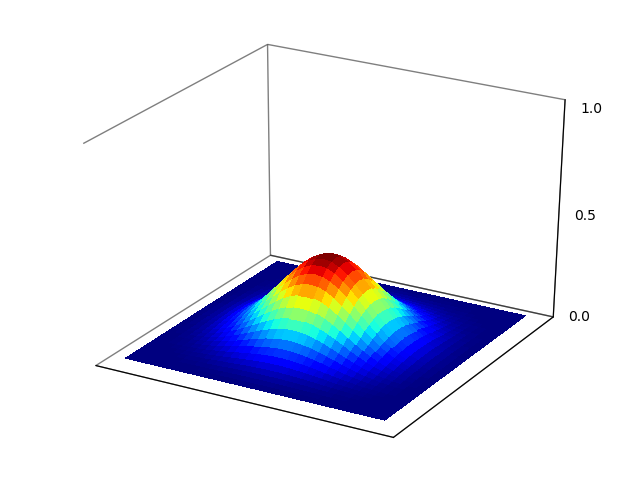
\includegraphics[width=0.3\columnwidth]{Figures/LME_5_0_Shape_Fun}
    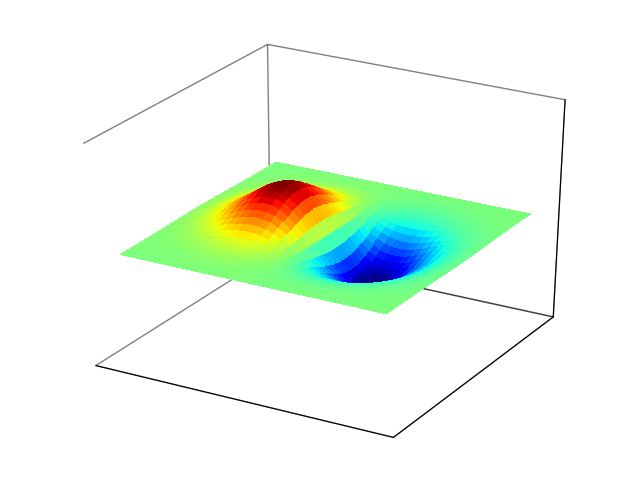
\includegraphics[width=0.3\columnwidth]{Figures/LME_5_0_Shape_Fun_dx}
    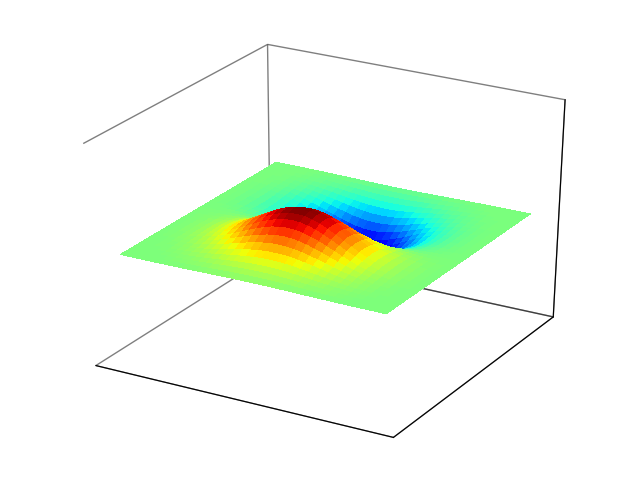
\includegraphics[width=0.3\columnwidth]{Figures/LME_5_0_Shape_Fun_dy}
    \label{fig:LME_5.0_Shape_Fun}
  }
  \caption{Local max-ent shape functions for a two-dimensional
    arrangement of nodes, and spatial derivatives for several values
    of $\gamma = \beta/h^2$.}
  \label{fig:LME_MPM}
\end{figure}

Since  $p_I$  is defined in the entire domain, in practice, the
function $\exp(-\beta \vec{r} )$ truncated  by  a given tolerance,
10$^{-6}$, for example,  would ensure a reasonable range of
neighbours, see \cite{Arroyo2006} for details. This tolerance defines
the limit values of the influence radius and is used thereafter to
find the neighbour nodes of a given integration point. Regarding this
aspect an important note in the implementation of this interpolation
technique in the MPM is 

In this research and in \cite{Arroyo2006}, $\Beta$ is a scalar as the
influence area of the shape function is controlled by the Euclidean
norm, therefore the search area is geometrically a circle in 2D, or a
sphere in 3D. Building upon the idea of anisotropic shape functions,
\cite{Kochmann2019} introduced an enhanced version of the original
local max-ent scheme, which uses an anisotropic support to deal with
tensile inestability. Nonetheless this is out of the scope of the
present document but will be incorporated in future research.

\section{Application to linear elasticity dynamic problems.}
\label{sec:Application-linear-elasticity-dynamic-problems}

This section is devoted to test the ability of both predictor-corrector
time integration scheme and the local \textit{max-ent} approximants to
overcome spurious oscillations due to the grid crossing and high
frequency loads under the context of the MPM.

\subsection{Dyka bar}
\label{sec:dyka-bar}

High frequency , the benchmark proposed by Dyka \& Ingel
(1995)\cite{Dyka1995} is considered to illustrate the
capacity of the proposed time integration algorithm to avoid velocity
fields instabilities.

In the one-dimensional bar sketched in the figure \ref{fig:Dyka_Bar},
the left end of the bar is fixed and the right and an initial velocity
$v_0 = 5\ m/s$ is given to the last quarter of it in the x positive
direction. The length of it is 0.1333 meters with an unit section.

\begin{figure}\sidecaption
  \centering
  \resizebox{\hsize}{!}{
    \begin{tikzpicture} 
  \scaling{2}; 
  % Nodos 
  \point{a}{0}{1};
  \point{b}{3.75}{1};
  \point{c}{5}{1};
  % Barras
  \beam{2}{a}{b};
  \beam{2}{b}{c};
  % Apoyos
  \support{3}{a}[270];
  % Fuerzas
  \lineload{4}{b}{c}[1][0.2];
  \notation{5}{b}{c}[$5\ m/s$][.5][below][2];
  % Nombres de nodos
  \notation{1}{a}{A}[below right];
  \notation{1}{b}{B}[below right];
  \notation{1}{c}{C}[below right];
  % Cotas
  \dimensioning{1}{a}{b}{0.5}[{\unit[3/4]{L}}];
  \dimensioning{1}{b}{c}{0.5}[{\unit[1/4]{L}}];
\end{tikzpicture}
}
  \caption{Geometrical description of the Dyka \cite{Dyka1995} bar.}
  \label{fig:Dyka_Bar}
\end{figure}

The elastic parameters consider for this test are:
\begin{itemize} 
\item  Density : $7833\ kg/m3$
\item  Poisson ratio : $0$
\item  Elastic modulus : $200 \cdot 10^9\ Pa$
\end{itemize}

The boundary conditions are:
\begin{equation}
  \label{eq:3}
  \sigma \rvert_{x=L} = 0 \quad , \quad v \rvert_{x=0} = 0
\end{equation}

The total simulation time is 0.0002 seconds, a direct consequence of
that is we let the elastic wave generated travel thorough the bar
(from A to C and back to A) at least four times. For the spatial
discretization we will set a mesh size of 3.3325 millimeters. The
initial mesh will be composed by a single particle in the center of
the element.

Regarding this, here we give one consideration to properly modellize
this benchmark under the MPM framework. Notice that the free border of
the bar has a horizontal displacement of 0.033 millimeters, therefore
a computational domain with an extra gap of 0.033 millimeters is
required in order to accommodate the unconstrained displacement of the
particles in the left border of the bar. Here below the time step is
controlled by the courant number, in this case, we adopt a middle
value of it (CFL=0.5) as a compromise between stability and numerical
accuracy.  

The analytical solution in terms of velocity
\ref{fig:vel_analytics_dyka}, and stress
\ref{fig:stress_analytics_dyka} can be found in the appendix
\ref{app:analytical_sol} given by the Method of characteristics.

\begin{figure}\sidecaption
  \centering
  \resizebox{\hsize}{!}{
    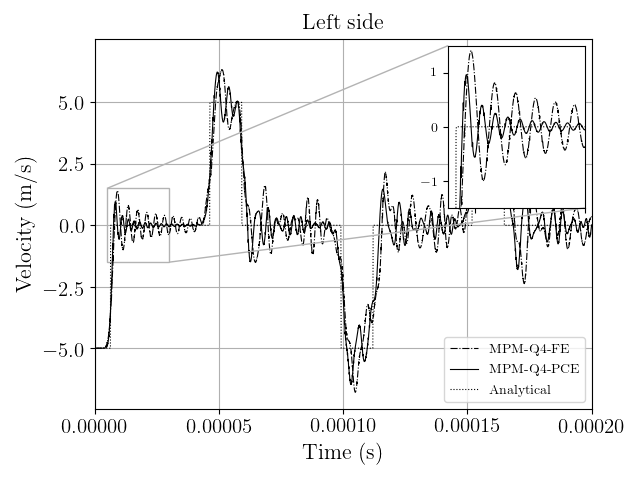
\includegraphics[width=\textwidth]{./Figures/Velocity_FE_vs_PCE_CFL_05}
  }
  \caption{Velocity evolution at the point in the bar left side.}
  \label{fig:Dyka-PCE-FE}
\end{figure}

\begin{figure}\sidecaption
  \centering
  \resizebox{\hsize}{!}{
    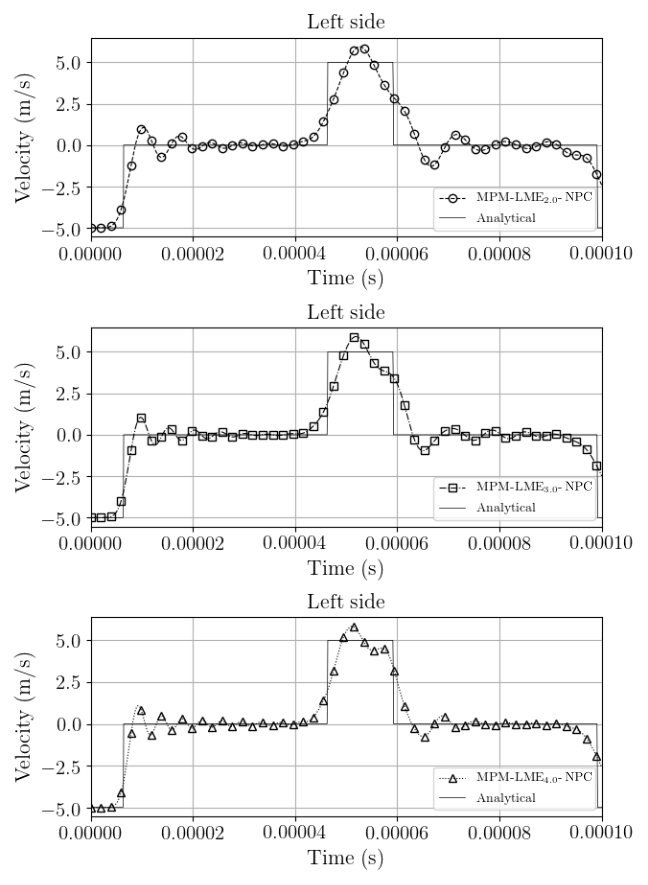
\includegraphics[width=\textwidth]{./Figures/Velocity_LME_gamma_comparative}
  }
  \caption{Velocity evolution at the point in the bar left side.}
  \label{fig:Dyka-LME-gamma}
\end{figure}

\begin{figure}\sidecaption
  \centering
  \resizebox{\hsize}{!}{
    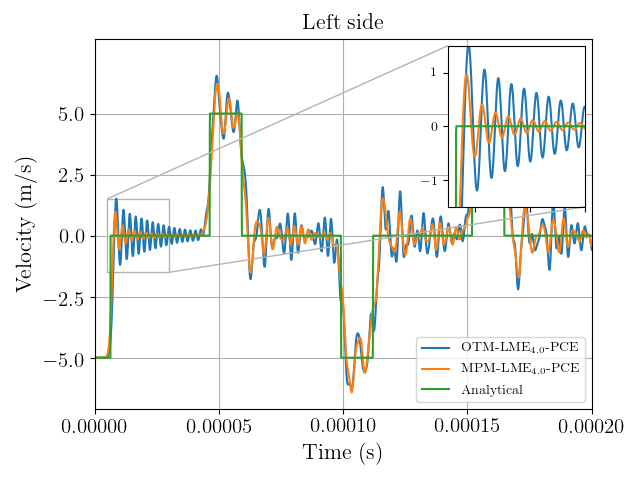
\includegraphics[width=\textwidth]{./Figures/Velocity_MPM_vs_OTM_Dyka}
  }
  \caption{Velocity evolution at the point in the bar left side.}
  \label{fig:Dyka-OTM-MPM}
\end{figure}

For the convergence analysis, the root-mean-square (RMS) error in the
velocity field is computed. RMS error is defined as follows

\begin{equation}
  \label{eq:RMS}
  RMS = \sqrt{\frac{1}{N} \sum^{N}_p \left( \vect{v}_p - \hat{\vect{v}}_p \right)^2},
\end{equation}

where $\vect{v}_p$ and $\hat{\vect{v}}_p$ are respectively the analytical and
numerical solutions evaluated in the final time step in the position
of each particle.


\begin{figure*}\sidecaption
  \centering
  \resizebox{\hsize}{!}{
    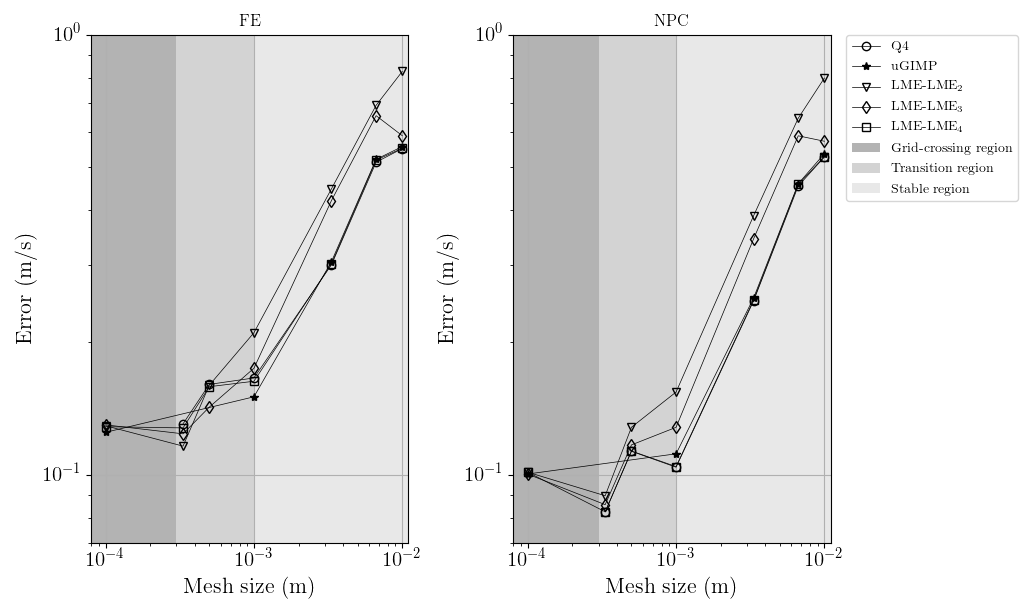
\includegraphics[width=\textwidth]{./Figures/Error_evol}
  }
  \caption{Velocity evolution at the point in the bar left side.}
  \label{fig:Dyka-error-evol}
\end{figure*}


\subsection{Andersen block}
\label{sec:andersen-block}

In order to test the ability of this interpolation technique to deal
with grid crossing instabilities we will simulate the vertical
compression of a square block (10 by 10 meters) of soft soil sketched
in figure \ref{fig:block} and loaded using an incremental gravitation scheme.

\begin{figure}\sidecaption
  \centering
  \resizebox{\hsize}{!}{
    \begin{tikzpicture} 
  \scaling{1};
  
% Nodos
\point{1}{0}{10};
\point{2}{2}{10};
\point{3}{0}{8};
\point{4}{2}{8};
\point{5}{4}{10};
\point{6}{0}{6};
\point{7}{2}{6};
\point{8}{4}{8};
\point{9}{4}{6};
\point{10}{6}{10};
\point{11}{0}{4};            
\point{12}{2}{4};            
\point{13}{6}{8};            
\point{14}{4}{4};            
\point{15}{6}{6};            
\point{16}{8}{10};            
\point{17}{0}{2};            
\point{18}{2}{2};            
\point{19}{8}{8};            
\point{20}{6}{4};            
\point{21}{4}{2};            
\point{22}{8}{6};            
\point{23}{0}{0};            
\point{24}{10}{10};            
\point{25}{6}{2};            
\point{26}{8}{4};
\point{27}{2}{0};            
\point{28}{10}{8};            
\point{29}{4}{0};            
\point{30}{10}{6};            
\point{31}{8}{2};            
\point{32}{6}{0};            
\point{33}{10}{4};            
\point{34}{8}{0};            
\point{35}{10}{2};            
\point{36}{10}{0};

% Barras
\beam{2}{27}{18};
\beam{2}{18}{17};
\beam{2}{17}{23};
\beam{2}{23}{27};
  
\beam{2}{29}{21};
\beam{2}{21}{18};
\beam{2}{18}{27};
\beam{2}{29}{27};

\beam{2}{32}{25};
\beam{2}{25}{21};
\beam{2}{21}{29};
\beam{2}{32}{29};

\beam{2}{34}{31};
\beam{2}{31}{25};
\beam{2}{25}{32};
\beam{2}{34}{32};

\beam{2}{36}{35};
\beam{2}{35}{31};
\beam{2}{31}{34};
\beam{2}{36}{34};

%%%%%%%%%%%%%%%%
\beam{2}{18}{12};
\beam{2}{12}{11};
\beam{2}{11}{17};
\beam{2}{18}{17};

\beam{2}{21}{14};
\beam{2}{14}{12};
\beam{2}{12}{18};
\beam{2}{21}{18};

\beam{2}{25}{20};
\beam{2}{20}{14};
\beam{2}{14}{21};
\beam{2}{25}{21};

\beam{2}{31}{26};
\beam{2}{26}{20};
\beam{2}{20}{25};
\beam{2}{31}{25};

\beam{2}{35}{33};
\beam{2}{33}{26};
\beam{2}{26}{31};
\beam{2}{35}{31};

%%%%%%%%%%%%%%%%
\beam{2}{12}{7};
\beam{2}{7}{6};
\beam{2}{6}{11};
\beam{2}{12}{11};

\beam{2}{14}{9};
\beam{2}{9}{7};
\beam{2}{7}{12};
\beam{2}{14}{12};

\beam{2}{20}{15};
\beam{2}{15}{9};
\beam{2}{9}{14};
\beam{2}{20}{14};

\beam{2}{26}{22};
\beam{2}{22}{15};
\beam{2}{15}{20};
\beam{2}{26}{20};

\beam{2}{33}{30};
\beam{2}{30}{22};
\beam{2}{22}{26};
\beam{2}{33}{26};

%%%%%%%%%%%%%%%%
\beam{2}{7}{4};
\beam{2}{4}{3};
\beam{2}{3}{6};
\beam{2}{7}{6};

\beam{2}{9}{8};
\beam{2}{8}{4};
\beam{2}{4}{7};
\beam{2}{9}{7};

\beam{2}{15}{13};
\beam{2}{13}{8};
\beam{2}{8}{9};
\beam{2}{15}{9};

\beam{2}{22}{19};
\beam{2}{19}{13};
\beam{2}{13}{15};
\beam{2}{22}{15};

\beam{2}{30}{28};
\beam{2}{28}{19};
\beam{2}{19}{22};
\beam{2}{30}{22};

%%%%%%%%%%%%%%%%
\beam{2}{4}{2};
\beam{2}{2}{1};
\beam{2}{1}{3};
\beam{2}{4}{3};

\beam{2}{8}{5};
\beam{2}{5}{2};
\beam{2}{2}{4};
\beam{2}{8}{4};

\beam{2}{13}{10};
\beam{2}{10}{5};
\beam{2}{5}{8};
\beam{2}{13}{8};

\beam{2}{19}{16};
\beam{2}{16}{10};
\beam{2}{10}{13};
\beam{2}{19}{13};

\beam{2}{28}{24};
\beam{2}{24}{16};
\beam{2}{16}{19};
\beam{2}{28}{19};

% Bottom
\support {1}{23}[315];
\support {1}{27}[0];
\support {1}{29}[0];
\support {1}{32}[0];
\support {1}{34}[0];
\support {1}{36}[45];

% \support {2}{23}[270];
\support {2}{1}[270];
\support {2}{3}[270];
\support {2}{6}[270];
\support {2}{11}[270];
\support {2}{17}[270];

\support {2}{24}[90];
\support {2}{28}[90];
\support {2}{30}[90];
\support {2}{33}[90];
\support {2}{35}[90];
% \support {2}{36}[90];

% Gravity
\point{g}{12}{5};
\load{1}{g}[90][3][0];

% Cotas
\dimensioning{1}{23}{36}{-1.5}[$10~m$];
\dimensioning{2}{23}{1}{-1.5}[$10~m$];


\end{tikzpicture}


% % Apoyos
% \support{3}{c}[90];
% % Fuerzas
% \lineload{4}{b}{a}[1][0.2];
% \notation{5}{a}{b}[$-5\ m/s$][.5][below][2];
% % Nombres de nodos
% \notation{1}{a}{A}[below left];
% \notation{1}{b}{B}[below left];
% \notation{1}{c}{C}[below left];
% % Cotas
% \dimensioning{1}{a}{b}{0.5}[{\unit[1/4]{L}}];
% \dimensioning{1}{b}{c}{0.5}[{\unit[3/4]{L}}];


% End Elements
}
  \caption{Geometrical description of a soil block }.}
  \label{fig:block}
\end{figure}

This test was taken from Andersen (2009)\cite{thesis_Andersen_2009}. The
elastic parameters consider for this test are: 
\begin{itemize} 
\item  Initial density : $6\cdot 10^3\ kg/m^3$
\item  Poisson ratio : $0$
\item  Elastic modulus : $5\ MPa$
\end{itemize}
The gravity force is a apply as an external force according to the
equations \eqref{eq:particle_body_forces},
\eqref{eq:nodal_external_forces}. Using a total time period of T (20
seconds) to apply the gravity, it is increased from 0 to 9.81$m/s$
with a sinus function until T/2 and then maintained constant until T
in order to arrive to a state of equilibrium, 
\begin{equation}
  \label{eq:gravity-load-block}
 \mathbf{g}(t) = \left\{
    \begin{array}{ll}
      0.5 \mathbf{g} (\sin(\frac{2t \pi}{T} - \frac{\pi}{2})+1)  & \mbox{if } t \leq T/2 \\
      \mathbf{g} & \mbox{if } t > T/2
    \end{array}
  \right.
\end{equation}

In order to get a stable solution, we will adopt a time step conducted
by a Courant number of 0.1. On the other hand, the explicit predictor-corrector
scheme is here employed looking forward getting better results. For the
initial spatial discretization we will employ four particles per cell
($\Delta x = 2\ m$). The initial setting of particles inside of the
cell changes according to the interpolation technique adopted. For the
bi-linear shape functions (Q4) and the LME shape functions, the initial
position corresponds to the location of the gauss-points in a standard
quadratic finite element. For the uniform-GIMP (uGIMP) shape function
the initial position of each particle is located in the center of each
voxel, due to the fact that in the initial situation, the voxel domain
should not overlap each others, Steffen {\it et al.}
(2008)\cite{Steffen2008}. Figure \ref{fig:vertical-displacement-block}
shows the vertical displacement evolution of a point in the free
surface of the block.
\begin{figure}\sidecaption
  \centering
  \resizebox{\hsize}{!}{
    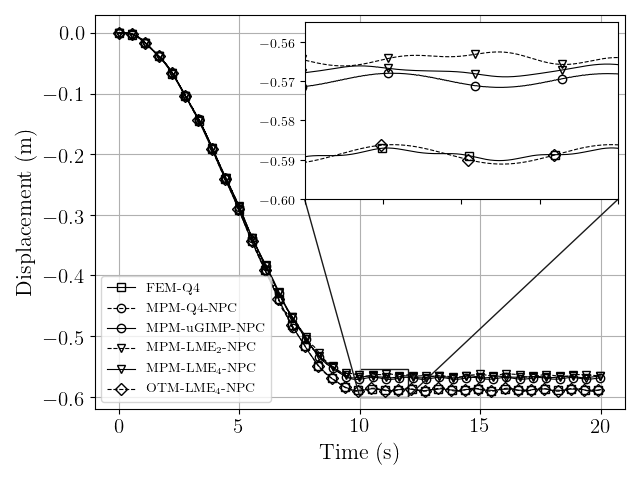
\includegraphics[width=\textwidth]{./Figures/Block_CFL_01_Comparative}
  }
  \caption{Comparative of the vertical displacement evolution in a
    point located in the free surface employing different
    interpolation schemes and numerical techniques.} 
  \label{fig:vertical-displacement-block}
\end{figure}

As we can see the simulation using the Q4 interpolation technique
turns out to be unstable and in the second 15 it fails. The uGIMP
simulation is more stable than the one performed by the Q4. Despite
this is still unstable and could trigger severe oscillations if we
pretend to simulate non-linear materials. The LME simulation was
performed using two kinds of shape functions, one with a low value of
the dimensionless parameter, $\gamma = 0.8$, and other with a larger
value of it, $\gamma = 3.0$. Notice that the results are both
stable, but the larger values of $\gamma$ give us a very stable
solution. This is due to the fact that with larger value of $\gamma$,
the shape functions behaves in a similar way to the FEM, which performs
very accurate in those cases with a reasonable mesh distorsion, and
with a lower value it behaves in a similar way to the uGIMP. This
behaviour was noticed previously by \cite{Arroyo2006}, were authors
highlight how by adjusting the spatial variation of $\beta(\vect{x})$,
it is possible to select regions of the domain of analysis which are
treated by finite elements and regions that are treated in the style
of meshfree methods, with seamless transitions between those regions.

Figure \ref{fig:Block-LME3} shows the evolution of the vertical stress
during the loading process. The result is physically realistic as
stress increments linearly from the top to the bottom of the specimen,
and the value of the vertical stress in a material point located in
the bottom of the specimen oscillates centered in $5.2 MPa$, which is
the analytic value given by $\sigma_{yy} = \rho g h_y$. 

\begin{figure}
  \centering
  %%%%%%%%%%%%%%%%%%%%%%%%%%%%%%%%%%%%%%%%%%%%%% 
  \subfloat[t = 0 seconds.]{
    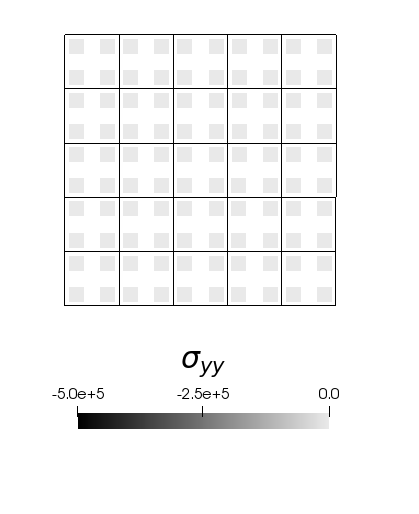
\includegraphics[width=0.8\columnwidth]{Figures/Block_LME3_PCE_a_t0}
    \label{fig:Block-LME3-PCE-t0}
  }
  %%%%%%%%%%%%%%%%%%%%%%%%%%%%%%%%%%%%%%%%%%%%%% 
  \qquad
  %%%%%%%%%%%%%%%%%%%%%%%%%%%%%%%%%%%%%%%%%%%%%% 
  \subfloat[t = 5 seconds.]{
    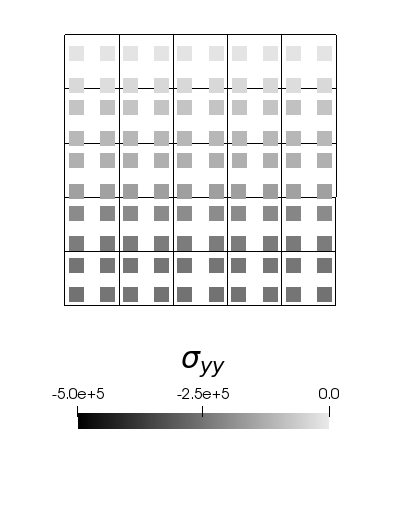
\includegraphics[width=0.8\columnwidth]{Figures/Block_LME3_PCE_b_t025}
    \label{fig:Block-LME3-PCE-t025}
  }
  %%%%%%%%%%%%%%%%%%%%%%%%%%%%%%%%%%%%%%%%%%%%%%
  \qquad
  %%%%%%%%%%%%%%%%%%%%%%%%%%%%%%%%%%%%%%%%%%%%%% 
  \subfloat[t = 20 seconds]{
    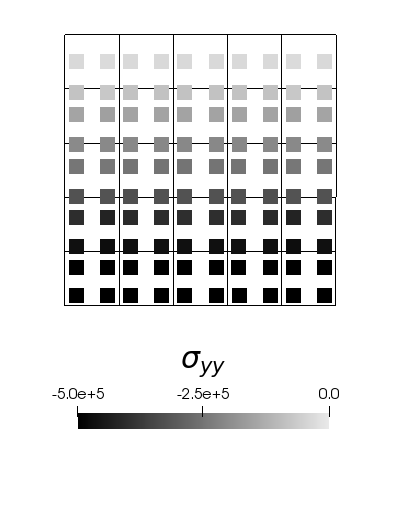
\includegraphics[width=0.8\columnwidth]{Figures/Block_LME3_PCE_c_t1}
    \label{fig:Block-LME3-PCE-t1}
  }
  %%%%%%%%%%%%%%%%%%%%%%%%%%%%%%%%%%%%%%%%%%%%%% 
  \caption{Vertical normal stress and position of material points
    during the loading process for a soft soil ($E = 5\ MPa$, $\rho_0
    = 6\cdot 10^3\ kg/m^3$). Numerical parameters considered for the
    simulation are : Local \textit{max-ent} shape function $\gamma =3$
    and explicit PC scheme with CFL 0.1.}
  \label{fig:Block-LME3}
\end{figure}


% \subsection{MPM versus OTM}
% \label{sec:mpm-versus-otm}

% MPM \cite{Sulsky1994} and OTM
% models to avoid tensile instabilities. Here we employ our in-house
% codes for both MPM and OTM simulations.

% The results are provided for the explicit predictor-corrector version
% of the MPM scheme (Algorithm \ref{alg:PCE-algorithm}) and OTM
% algorithms. For MPM, piecewise-linear, uGIMP and \textit{max-ent}
% basis functions are employed. The OTM algorithm is used only with
% \textit{max-ent} shape functions.

% \begin{figure*}\sidecaption
%   \centering
%   \resizebox{0.7\hsize}{!}{
%     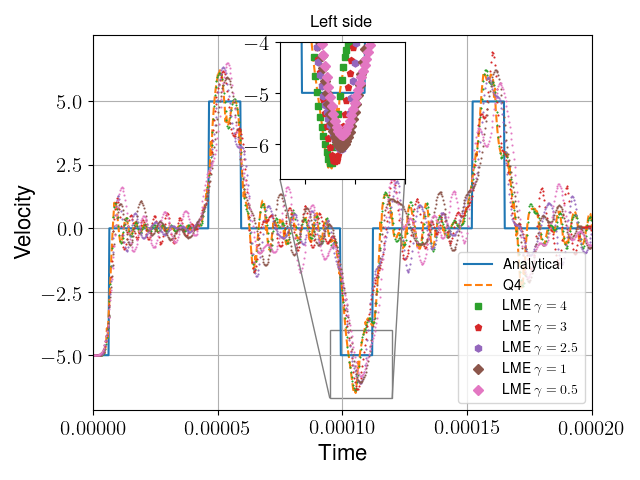
\includegraphics[width=\textwidth]{./Figures/Velocity-Comparative}
%   }
%   \caption{Velocity evolution at the point in the bar left side.}
%   \label{fig:Dyka-MPM-uGIMP-LME}
% \end{figure*}


\section{Conclusions}
\label{sec:conclusions}
We have developed a new time integration scheme for the MPM, and
proved how local \textit{max-ent} arise as a promising tool to
overcome the grid-crossing error.

adapt the value of $\beta$ to solve the equations fem-like of
meshfree-like depending of how behaves the region

This alternative technique overcome the constriction of the GIMP to
regular mesh.

The time integration here proposed mitigates the presence of wiggles
and overshot

future research :
localization of the local max ent

predictor-corrector for high dynamic problems like impact or
collisions 

\begin{acknowledgements}
If you'd like to thank anyone, place your comments here
and remove the percent signs.
\end{acknowledgements}

%
\section*{Conflict of interest}
%
The authors declare that they have no conflict of interest.


\appendix
\section{The analytical solution of the 1D Dyka benchmark}
\label{app:analytical_sol}

For the derivation of this analytical solution we will consider  the
dynamic behaviour of a 1D elastic bar. The governing equations are the
following: (i) The balance of linear momentum,
\begin{equation}
  \label{eq:1D-balance-linear-momentum}
  \rho\ \Deriv{v}{t} = \Deriv{\sigma}{x},
\end{equation}
where $\sigma$ is the stress value, $\rho$ is the density, and 
$v$ is the velocity. (ii) The constitutive model, which for convenience of the
following developments will be written in terms of displacement and
velocities as, 
\begin{equation}
  \label{eq:1D-constitutive-equation}
  \Deriv{\sigma}{t} = E \Deriv{\varepsilon}{t},
\end{equation}
where $E$ is the elastic modulus. (iii) The compatibility equation
also in terms of the velocity field,
\begin{equation}
  \label{eq:CompatibilityEquation_e}
  \Deriv{\varepsilon}{t} = \Deriv{v}{x}.
\end{equation}
Next for simplicity, we will introduce \eqref{eq:CompatibilityEquation_e} in 
\eqref{eq:1D-constitutive-equation}, so we get the following system of equations,
\begin{align}
  \label{eq:1D-balance-linear-momentum-II}
  \Deriv{v}{t} &= \frac{1}{\rho}\ \Deriv{\sigma}{x}, \\
  \label{eq:1D-constitutive-equation-II}
  \Deriv{\sigma}{t} &= E\ \Deriv{v}{x}.
\end{align}

Introducing \eqref{eq:1D-constitutive-equation-II} in
\eqref{eq:1D-balance-linear-momentum-II} and expressing the remaining
equation in terms of the displacement, we reach the 1D wave
equation for linear elastic materials,
\begin{equation}
  \label{eq:1D-wave-elastic}
  \Deriv[2]{u}{t} = \frac{E}{\rho}\ \Deriv[2]{u}{x} = c^2\ \Deriv[2]{u}{x}
\end{equation}
where we have introduced the wave celerity $c$ as,
\begin{equation}
  \label{eq:1D-elastic-wave-celerity}
  c = \sqrt{\frac{E}{\rho}}
\end{equation}
Alternative, rearranging both equations
\eqref{eq:1D-balance-linear-momentum-II} and
\eqref{eq:1D-constitutive-equation-II} it is possible to join them in a
single system of equations as,
\begin{equation}
  \label{eq:System-stress-velocity}
  \Deriv{}{t} \left[
    \begin{array}{c}
      \sigma \\
      v
    \end{array}
  \right] + \left[
    \begin{array}{cc}
      0 & - E \\
      - 1/\rho & 0 
    \end{array} \right] \left[
    \begin{array}{c}
      \Deriv{\sigma}{x} \\
      \Deriv{v}{x}
    \end{array}
  \right] = \Vector{0}.
\end{equation}
This expression can be written in a more compact format as,
\begin{equation}
  \label{eq:System-stress-velocity-II}
  \Deriv{\Vector{\phi}}{t} + \Matrix{A}\Deriv{\Vector{\phi}}{x} = \Vector{0}
\end{equation}
where both variables are joined in a single vectorial variable
$\Vector{\phi}$ and $\Matrix{A}$ in coupling matrix between both equations,
\begin{equation*}
  \Vector{\phi} = \left[
    \begin{array}{c}
      \sigma \\
      v
    \end{array}
  \right],\quad 
  \Matrix{A} =  \left[
    \begin{array}{cc}
      0 & - E\\
      - 1/\rho & 0 
    \end{array} \right].
\end{equation*}
Note that the nature of \label{eq:eq:System-stress-velocity-II} is still
hyperbolic despite the fact it does not have a second order
temporal derivative as \eqref{eq:1D-wave-elastic}. A proof of this can
be easily obtained if we get the zeros of the hypersurface defined by
\eqref{eq:1D-wave-elastic}. And later the eigenvalues of $\Matrix{A}$
in \eqref{eq:System-stress-velocity-II}. In both cases, eigenvalues
are real and distinct ($\lambda = \pm \sqrt{\frac{E}{\rho}}$),
therefore the system is called strictly hyperbolic.

For a more general description in the following, we will assume that $\Matrix{A}$ has $n$
different eigenvalues $\{ \lambda_1, \lambda_2, \ldots, \lambda_i, \ldots
\lambda_n \}$ and $n$ eigenvectors $\{ \vec{x}^1, \vec{x}^2, \ldots,
\vec{x}^i, \ldots \vec{x}^n \}$ satisfying that $\tens{A} \vec{x} =
\lambda \vec{x} $. Now we introduce the matrix $\Matrix{P}$ whose columns are the $n$
eigenvalues $\Vector{x}$
\begin{equation}
  \label{eq:P-matrix}
\Matrix{P} = \{ \vec{x}^1, \vec{x}^2, \vec{x}^3, \ldots \vec{x}^n \}.
\end{equation}
Diagonalizing $\Matrix{A}$ using $\Matrix{P}$ we get
\begin{equation}
  \label{eq:Lambda-matrix}
  \Lambda = \Matrix{P}^{-1} \Matrix{A}\ \Matrix{P},
\end{equation}
where $ \Lambda_{ii} = \lambda_i$. Next we will define a vector $\Vector{\Re}$ such that:
\begin{equation}
  \label{eq:Riemann-definition}
  \Vector{\phi} = \Matrix{P}\ \Vector{\Re}
\end{equation}
we will assume to be integrable. Expanding the above expression with
the chain rule and passing the matrix $\Matrix{P}$ to left hand side
of the equality we get,
\begin{equation}
  \label{eq:Riemann-II}
  d \vec{\Vector{\Re}} = \Deriv{\Vector{\Re}}{t}dt + \Deriv{\Vector{\Re}}{x}dx =
  \tens{P}^{-1}\left(\Deriv{\phi}{t}dt + \Deriv{\phi}{x}dx \right)
\end{equation}
and setting the terms we get,
\begin{equation}
  \label{eq:Riemann-III}
  \Deriv{\Vector{\Re}}{t} = \Matrix{P}^{-1}\Deriv{\Vector{\phi}}{t},\quad 
  \Deriv{\Vector{\Re}}{x} = \Matrix{P}^{-1}\Deriv{\Vector{\phi}}{x}
\end{equation}
Next, if we multiply \eqref{eq:System-stress-velocity-II} by
$\Matrix{P}^{-1}$ we get:
\begin{equation}
  \label{eq:System-stress-velocity-III}
  \Matrix{P}^{-1}\Deriv{\Vector{\phi}}{t} + \left(\Matrix{P}^{-1}\Matrix{A}\Matrix{P}
  \right)\Matrix{P}^{-1} \Deriv{\Vector{\phi}}{x} = \Vector{0}
\end{equation}
finally introducing the expressions \eqref{eq:Riemann-III} we reach to
\begin{equation}
  \label{eq:System-stress-velocity-IV}
  \Deriv{\Vector{\Re}}{t} + \varLambda \Deriv{\Vector{\Re}}{x} = \Vector{0}  
\end{equation}
which consists of $n$ uncoupled equations as $\varLambda$ is
diagonal matrix as we can see in \eqref{eq:Lambda-matrix}. Each of this
equations are 1D scalar convective transport equations, with solutions
of the form:
\begin{equation}
  \label{eq:SystemEquations_sigma_v_VI}
  \Re^{(i)} = F^{(i)} \left(x - \lambda^{(i)} t \right)
\end{equation}

This uncoupled system, has, therefore, a set of $n$ characteristics.
These magnitudes $\Re_i$ which propagate along characteristics are
known as ``Riemann invariants'' of the problem. Here we have a 1D
configuration, so the domain is $\Omega : \left(0, L\right) x \left(0,
  T\right)$. For the closure of the problem we require:
\begin{itemize}
\item ``n'' initial conditions of the form $\Re_i (x,t=0) = h_i(x)$,
  where $i = {0, \ldots, n}$, and $h_i(x)$ is a vectorial function
  given by the physical variables of the problem.
\item ``n'' boundary conditions.
\end{itemize}

Now particularizing the previous equations for the 1D elastic bar
described in \cite{Dyka1995}, we get that the matrix $\Matrix{P}$
is the following:
\begin{equation*}
    \Matrix{P} =  \left[
    \begin{array}{cc}
      -\sqrt{E\rho} & \sqrt{E\rho}\\
       1 & 1 
    \end{array} \right]
\end{equation*}
and its inverse is:
\begin{equation*}
    \Matrix{P}^{-1} = \frac{1}{2\ \sqrt{E\rho}} \left[
    \begin{array}{cc}
      -1 & \frac{1}{\sqrt{E\rho}}\\
      1 & \frac{1}{\sqrt{E\rho}} 
    \end{array} \right]
\end{equation*}

And introducing the value of the inverse matrix $\Matrix{P}^1$ in the
Riemann definition \eqref{eq:Riemann-definition} we get the following
system of equations,
\begin{align}
  \label{eq:Riemann-I-1D-elastic-bar}
  &\Re^{I} = \frac{1}{2\sqrt{\rho E}}\left(-\sigma + v\ \sqrt{\rho E}
    \right)\\
  \label{eq:Riemann-II-1D-elastic-bar}
  &\Re^{II} = \frac{1}{2\sqrt{\rho E}}\left(\sigma + v\ \sqrt{\rho E} \right)
\end{align}

From \eqref{eq:Riemann-I-1D-elastic-bar} and
\eqref{eq:Riemann-II-1D-elastic-bar} we can obtain the values of the
stress and the velocity as:
\begin{equation}
  \label{eq:Riemann-stress-velocity}
  v = \Re^{I} + \Re^{II} \quad , \quad \sigma = \sqrt{E \rho}\left(\Re^{II} - \Re^{I} \right)
\end{equation}

The boundary conditions are in both cases of radiation as there is not
wave in-going from the exterior. So for the right side (fixed
boundary) we get the following conditions:
\begin{equation*}
  \Re^{II} = 0 \quad and \quad v_{x=L} = 0
\end{equation*}
Therefore $\sigma_{x=L} = -2\sqrt{\rho E}\ \Re^{I}$. And in the left side
(free boundary) we get the following conditions:
\begin{equation*}
  \Re^{I} = 0 \quad and \quad \sigma_{x=0} = 0
\end{equation*}
Therefore $v_{x=0} = 2\Re^{II}$. Finally, applying this conditions in
the elastic bar sketched in \ref{fig:Dyka_Bar}, is possible to obtain
the velocity history in the right side of the bar
\ref{fig:vel_analytics_dyka} and the stress in the last quarter side of the Dyka
bar \ref{fig:stress_analytics_dyka} as is demanded in \cite{Dyka1995}.

\begin{figure}\sidecaption
  \centering
  \resizebox{\hsize}{!}{
    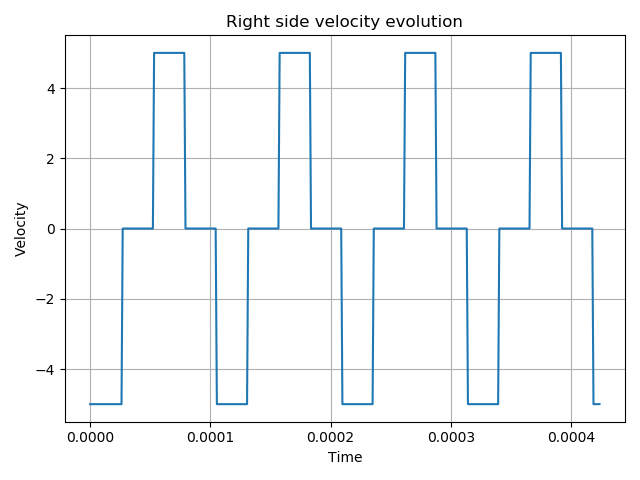
\includegraphics[width=\columnwidth]{Figures/1D_right_Velocity.png}
  }
  \caption[Velocities values in the right side of the Dyka
  bar]{Analytical solution for the velocity in the right side of the Dyka bar.}
  \label{fig:vel_analytics_dyka}
\end{figure}

\begin{figure}\sidecaption
  \centering
  \resizebox{\hsize}{!}{
    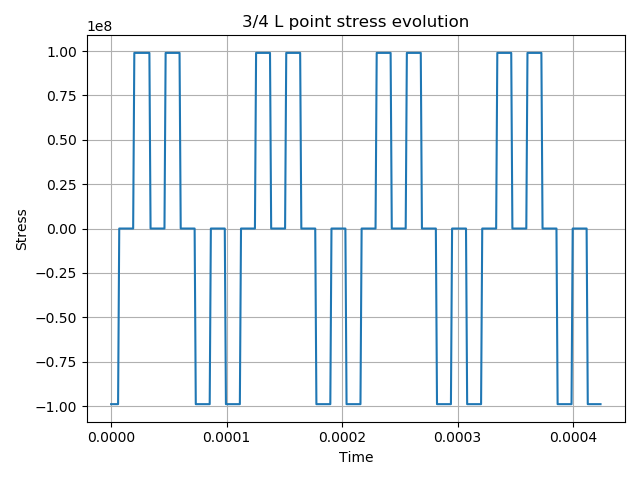
\includegraphics[width=\columnwidth]{Figures/1D_left_Stress.png}
  }
  \caption[Stress values in the last quarter side of the Dyka
  bar]{Analytical solution for the stress in the last quarter of the Dyka bar.}
  \label{fig:stress_analytics_dyka}
\end{figure}



% BibTeX users please use one of
%\bibliographystyle{spbasic}      % basic style, author-year citations
\bibliographystyle{spmpsci}      % mathematics and physical sciences
%\bibliographystyle{spphys}       % APS-like style for physics
\bibliography{Biblio.bib}   % name your BibTeX data base

\end{document}
% end of file template.tex


%%% Local Variables:
%%% mode: latex
%%% TeX-master: t
%%% End:

